\documentclass[sotsuron]{kuee}

\usepackage[dvipdfmx]{graphicx}
\usepackage{here}
\usepackage{amsmath}
\usepackage{bm}
\usepackage{multirow}


\title{DNAストレージにおけるナノポアシーケンサーの読み出し特性を考慮した誤り訂正手法}
\etitle{Error Correction Method Considering the Reading Characteristics of Nanopore Sequencers in DNA Storage}
\author{岩瀬 真太郎}
\eauthor{Shintaro Iwase}
\professor{佐藤 高史 教授}
% \course{京都大学大学院情報学研究科}
% \department{知能情報学専攻}
\date{令和8年2月10日}

%%% 本文
\begin{document}
\maketitle			% 表題を出力
\begin{eabstract}		% 英文要旨を出力
In today's information society, large amounts of digital data are generated 
every day, and the amount of data worldwide continues to grow explosively. 
DNA storage has emerged as a promising solution for long-term archival storage 
due to its high information density and durability. While nanopore sequencers 
offer advantages in reading long DNA sequences at high speeds, they suffer from 
lower accuracy compared to short-read sequencers, particularly with insertion 
and deletion errors. Although existing error-correcting codes have been proposed 
for DNA storage with capability to correct these errors, their decoding algorithms 
have not been optimized for the specific characteristics of nanopore sequencers.

This study aims to optimize existing error correction methods 
specifically for DNA storage systems using nanopore sequencers. The proposed 
method incorporates two key improvements: (1) optimization of reward and penalty 
parameters based on statistical transition matrices that model nanopore reading 
characteristics, and (2) integration of confidence scores from the basecaller's 
CTC (Connectionist Temporal Classification) output into the decoding process. 
Additionally, to address accuracy degradation with longer DNA sequences, we 
propose a segmentation-based encoding scheme that divides sequences into short 
segments with separators and reinitializes the hash function at segment boundaries.

Simulation results demonstrate that the proposed method improves 
both decoding efficiency and accuracy. The optimized decoding algorithm reduces 
heap search operations by 64-68\% and bit deletion rates by 76-83\% compared to 
the existing method. The segmentation scheme maintains stable decoding accuracy 
even for DNA sequences up to 15,000\,nt without significantly increasing computational 
complexity. 
% After Reed-Solomon outer decoding, the proposed method achieves a 77\% 
% error rate reduction at 0.75 coding rate compared to the existing method. These 
% results demonstrate that the proposed optimization makes nanopore sequencers more 
% practical and effective for DNA storage applications.

\end{eabstract}
\tableofcontents		% 目次を出力

\section{Introduction}
In today's highly digitized society, massive volumes of data are generated every day,
and the total amount of data worldwide continues to grow explosively.
According to a 2025 report, the global volume of digital data is estimated to reach
173.4 zettabytes, and is projected to grow to 527.5 zettabytes by 2029\cite{statista_worldwide_data_created}.
It is known that approximately 60\% of this data is cold data whose access frequency is extremely low\cite{dna_data_storage_alliance_2021_intro}.
Cold data includes information that must be retained for long periods due to legal or regulatory requirements,
as well as research data that may be analyzed in the future, and thus cannot simply be discarded.
Therefore, there is a strong demand for archival storage technologies that can store cold data for long periods
at low cost\cite{reinsel2017dataage2025,dna_data_storage_alliance_2021_intro}.

Recently, DNA data storage has attracted considerable attention as a next-generation archival storage technology.
In DNA storage, digital data is encoded into sequences over the four nucleotides
adenine (A), cytosine (C), guanine (G), and thymine (T), and stored in synthetically fabricated DNA molecules.
DNA offers extremely high durability that can support preservation over thousands of years under appropriate
environmental conditions, and its volumetric information density can in principle far exceed that of conventional media.
Consequently, DNA storage is regarded as a promising candidate for long-term archival storage of cold data
\cite{akash2024_applicable,Ceze2019,dna_data_storage_alliance_2021_intro}.

For reading data stored in DNA, DNA sequencers are used to determine the nucleotide sequences\cite{Ceze2019}.
Sequencing technologies are broadly classified into short-read sequencers, which target DNA fragments of
several tens to a few hundreds of base pairs (bp)\footnote{Abbreviation of base pair. It is used as a unit for the
length of double-stranded DNA. For single-stranded DNA, we use nucleotides (nt).},
and long-read sequencers, which can read DNA with lengths ranging from several hundreds to tens of thousands of bp\cite{Amarasinghe2020}.
Most prior work on DNA storage has assumed short-read sequencers based on sequencing-by-synthesis (SBS) technology\cite{SBS}.
SBS can read a large number of short DNA fragments in parallel with high accuracy,
but it can only handle sequences on the order of a few hundred bp at a time and tends to have long turnaround times\cite{SBS}.
In contrast, nanopore sequencers, one type of long-read sequencer, can directly read DNA of up to several hundred kilobases
at high speed, and are therefore more suitable for practical DNA-storage readout\cite{Amarasinghe2020}.
In this work, we focus on DNA storage systems that use nanopore sequencers for readout.

While nanopore sequencers can rapidly decode long DNA strands, their basecalling accuracy is lower than that of SBS-based
short-read sequencers, and in particular they suffer from frequent insertion and deletion errors\cite{Amarasinghe2020,Dorey2024}.
When employing nanopore sequencers for DNA storage, it is therefore crucial to design error-correcting codes that can
handle not only substitution errors but also insertion and deletion errors.

Previous work has proposed error-correcting codes for DNA storage that satisfy sequence constraints such as
homopolymer suppression and GC-content balancing, while being capable of correcting substitution, insertion,
and deletion errors.
Through simulations and experiments using synthesized DNA, it has been shown that petabyte-scale data can in principle
be reliably recovered even when the sequencing output contains up to about 10\% errors\cite{HEDGES}.
However, that work assumes short-read sequencers for readout and does not optimize the code or decoding algorithm
for the specific error characteristics of nanopore sequencers.
Moreover, it reports that the decoding performance degrades as the DNA strand length increases, implying that
further improvements are required when long-read sequencers such as nanopore devices are used to handle long strands.

In this paper, we propose an error correction method tailored to DNA storage systems that use nanopore sequencers for readout.
We optimize the decoding algorithm of an existing code by incorporating statistical characteristics of nanopore sequencing,
thereby improving both decoding efficiency and accuracy.
In addition, we modify the encoding process to mitigate the degradation of decoding performance when operating on
long DNA strands.
We evaluate the proposed method via end-to-end simulations, from binary encoding through nanopore-based readout
and decoding back to binary data.

\section{Encoding and Readout in DNA Storage}
% This chapter outlines nanopore-based DNA sequencing and
% HEDGES, an error-correcting code for DNA storage.
% It also summarizes the limitations of existing methods and motivates our work.
\subsection{Overview of DNA Storage} \label{dna_storage}
DNA storage encodes digital data into DNA sequences and stores it in synthetically synthesized DNA molecules.
% An overview of the data write and read pipeline in DNA storage is shown in Fig.~\ref{fig:dna_storage}.
% \begin{figure}
%     \begin{center}
%         
\includegraphics[width=150mm]{noimage.png}
%         \caption{Write and read pipeline of DNA storage}\label{fig:dna_storage}
%     \end{center}
% \end{figure}
The process of storing and retrieving data in DNA storage typically consists of the following steps:
\begin{enumerate}
  \item Encoding\\
  The binary data is first encoded into DNA sequences.
  % Various encoding schemes have been proposed,
  % including simple 2-bit-to-1-base mappings, table-based mappings between bit strings and sequences,
  % and HEDGES encoding described later\cite{Grass2015Robust,DNAFountain,HEDGES}.
  To suppress synthesis errors and ensure structural stability, sequence constraints must be imposed.
  Typical constraints include prevention of long homopolymers and keeping the GC content within a certain range\cite{Gervasio}.
  In addition to adding redundancy for correcting errors during decoding, robustness against errors introduced
  during sequencing must also be considered.
  \item Storage\\
  Based on the encoded sequences, synthetic DNA molecules are manufactured.
  To improve storage density and stability, it is common to keep the DNA in a dehydrated state\cite{landsman2023the}.
  Under such conditions, data is expected to remain readable for thousands of years\cite{Grass2015Robust}.
  \item Data readout\\
  To read out the stored data, the DNA is first extracted and then sequenced using DNA sequencers such as
  SBS-based devices or nanopore sequencers described in Section~\ref{nanopore}.
  Sequencing introduces three main types of errors:
  \begin{itemize}
    \item Substitution error: the read base is different from the original base.
    \item Insertion error: an extra base not present in the original sequence is inserted in the readout.
    \item Deletion error: a base present in the original sequence is missing in the readout.
  \end{itemize}
  The original binary data must be reconstructed from sequences containing these errors by applying
  suitable error-correction algorithms.
\end{enumerate}

\subsection{HEDGES} \label{hedges}
HEDGES (Hash Encoded, Decoded by Greedy Exhaustive Search) is an error-correcting scheme that satisfies DNA
sequence constraints while being robust to substitution, insertion, and deletion errors\cite{HEDGES}.
\subsubsection{Encoding} \label{hedges_encoding}
HEDGES processes data on a packet basis.
Each packet consists of 255 fixed-length DNA strands, where the strand length is a design parameter.
Encoding is performed in two stages: an outer Reed--Solomon (RS) code converts the input bitstream into a
redundant bitstream with error-correction capability, and an inner HEDGES encoder further maps this bitstream
into DNA sequences with additional redundancy.
Figure~\ref{fig:hedges_encoding} shows an overview of the HEDGES encoding process.
\begin{figure}
    \begin{center}
        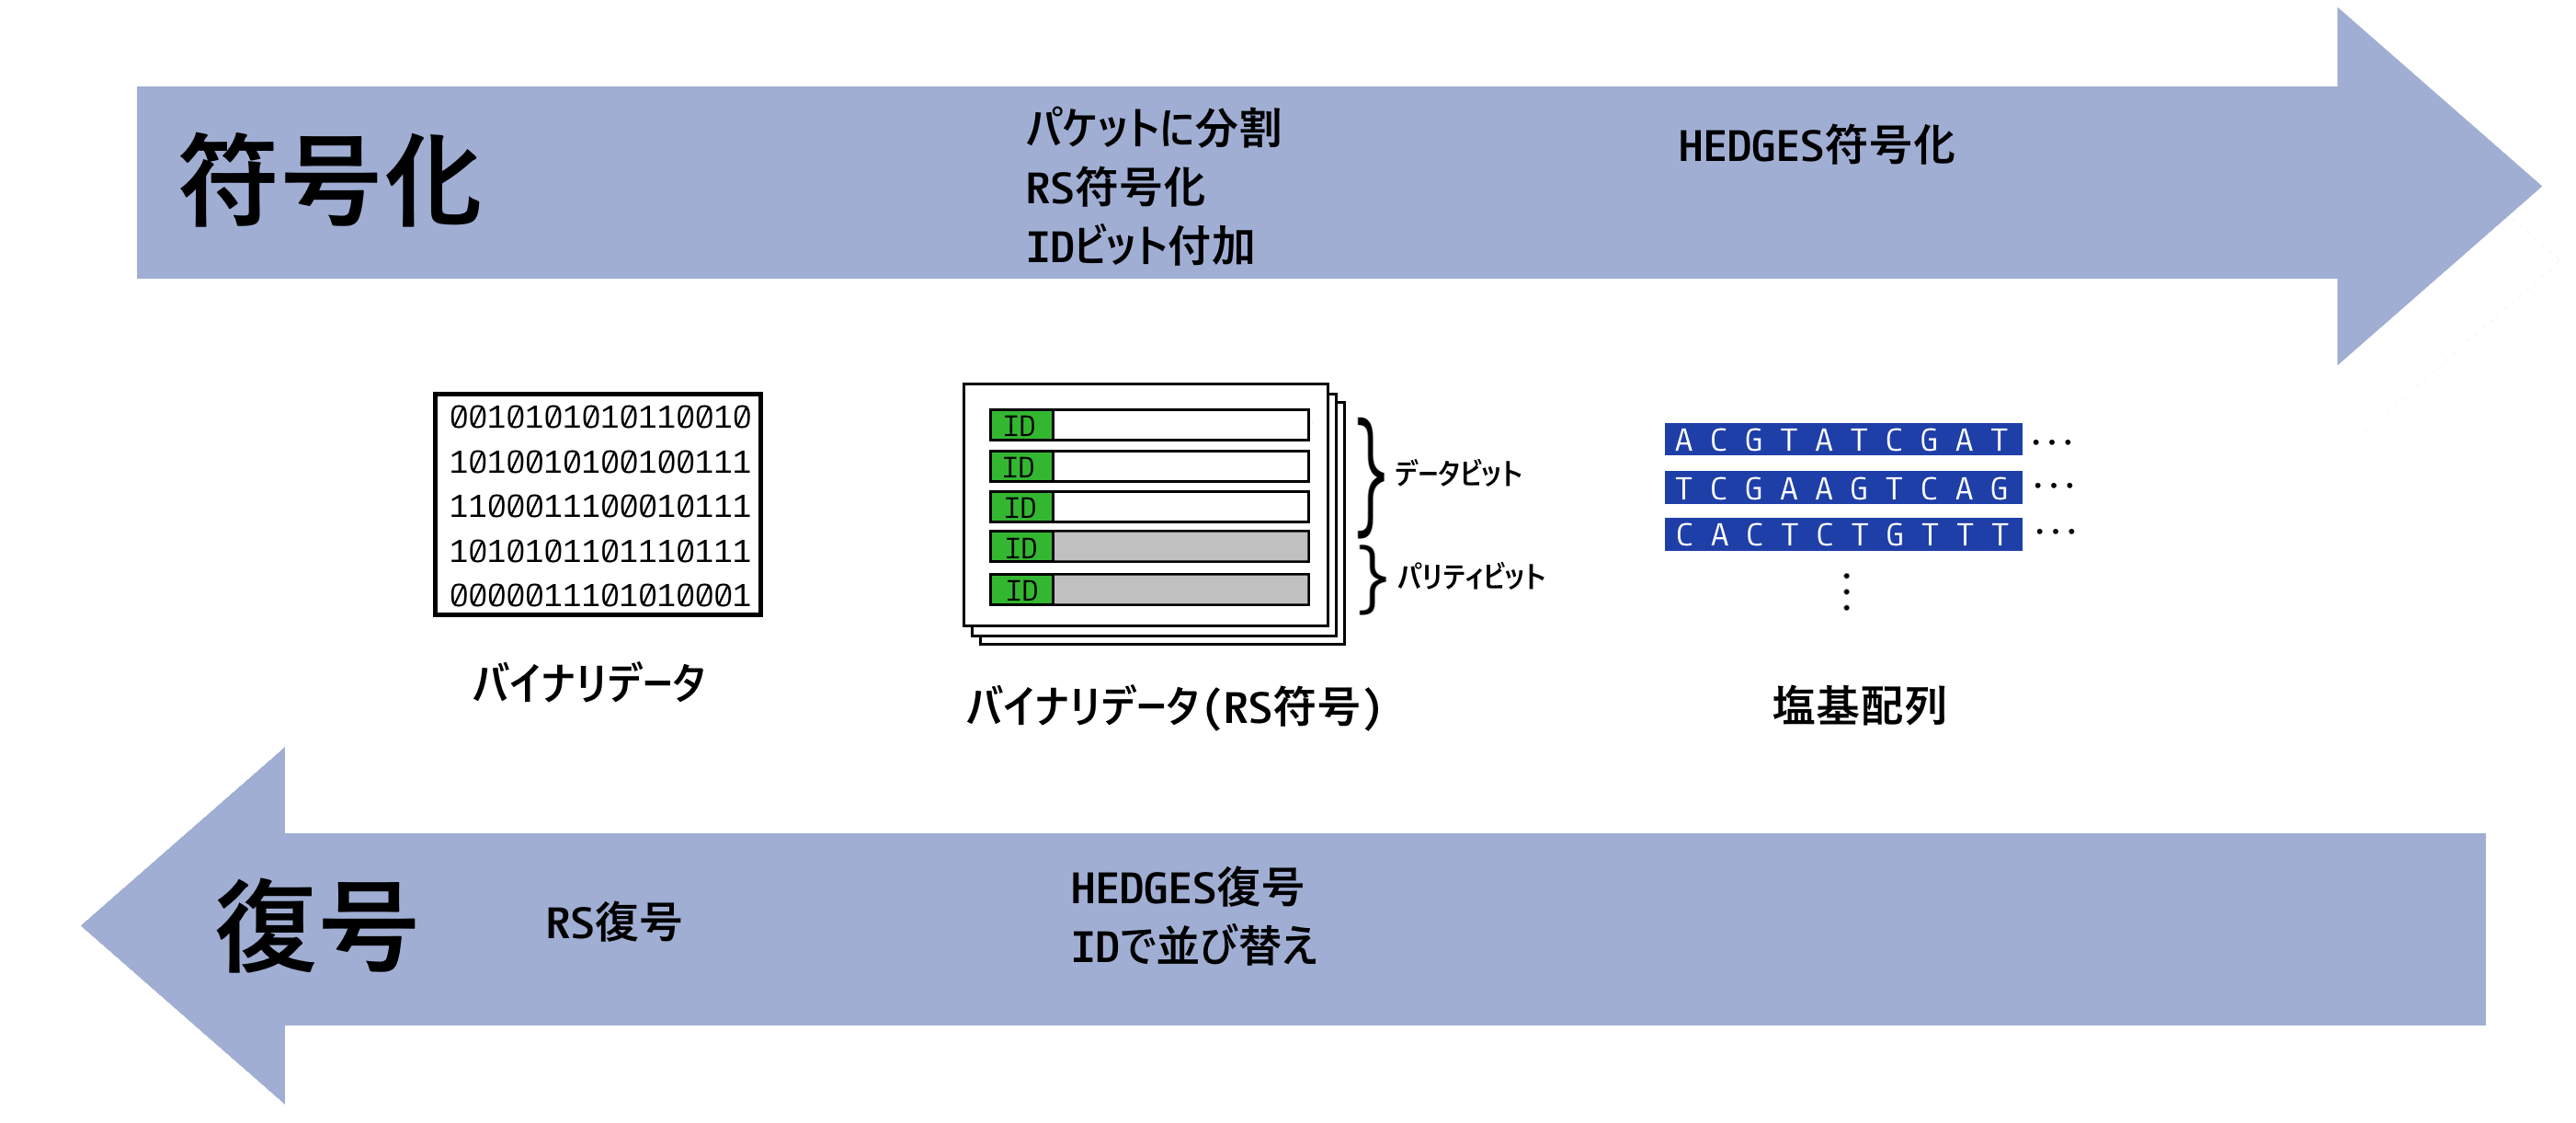
\includegraphics[width=150mm]{hedges.png}
    \caption{Overview of HEDGES encoding}\label{fig:hedges_encoding}
    \end{center}
\end{figure}
First, the binary data is divided into packets, and RS coding is applied to the bits of each packet to
obtain one RS codeword per packet.
The RS code is used as an outer code and ultimately corrects residual errors that remain after decoding
from DNA sequences back to bits.
Next, the inner HEDGES encoder is applied to the RS-coded bits to generate DNA sequences with additional redundancy.
An important feature of HEDGES is that the code rate for mapping bits to bases is configurable.
By lowering the rate, more redundancy is introduced and higher error-correction capability is obtained.

Below we describe the concrete encoding procedure of HEDGES.
Let the message bit sequence $\{b_i\}$ be given as
\begin{align}
  b_i, \quad i=0,1,2,\ldots, M, \quad b_i \in \{0,1\}
\end{align}
% 符号化率$r=0.5$では，
% 各ビット$b_i$に対して塩基$C_i$を割り当てればよい．
% \begin{align}
%   C_i, \quad i=0,1,2,\ldots M, \quad C_i \in \{C_i^*\}
% \end{align}
To realize arbitrary code rates, the number of bits assigned to each base is periodically varied between 0 and 2.
Thus, the bit sequence $\{b_i\}$ is partitioned into subsequences $v_i$ whose lengths range from 0 to 2 bits.
Examples of $v_i$ for code rates $r=0.750$, $r=0.500$, and $r=0.333$ are as follows:
\begin{align}
  r=0.750&: \quad v_0 = b_0b_1, \quad v_1 = b_2, \quad v_2 = b_3b_4, \quad v_3 = b_5, \quad v_4 = b_6b_7, \ldots \label{eq1} \\
  r=0.500&: \quad v_0 = b_0, \quad v_1 = b_1, \quad v_2 = b_2, \quad v_3 = b_3, \ldots \\
  r=0.333&: \quad v_0 = b_0, \quad v_1 = b_1, \quad v_2 = 0, \quad v_3 = b_2, \quad v_4 = b_3, \quad v_5 = 0, \ldots
\end{align}
Here, adjacent bits in Eq.~\eqref{eq1} represent a 2-bit value.
For $r=0.750$, the number of bits per base alternates between 2 and 1.
For $r=0.500$, each base carries 1 bit.
For $r=0.333$, the number of bits per base repeats in the pattern 1, 1, 0.
Let each subsequence $v_i$ be mapped to a base $C_i$ as
\begin{align}
  &C_i, \quad i=0,1,2,\ldots ,N, \quad C_i \in \{C_i^*\}
\end{align}
Here, $\{C_i^*\}$ denotes the set of admissible bases at position $i$ that satisfy the sequence constraints,
which is determined from the last few emitted bases.
For example, when a maximum homopolymer length is imposed, if the most recent output bases already form a homopolymer
of the maximum allowed length, the same base is excluded from the candidate set at the next position.
When constraining GC content, either \{A,T\} or \{C,G\} is removed from the candidate set depending on the local
GC ratio over the last several bases.
Thus, the cardinality $\#C_i^*$ varies in the range $0 < \#C_i^* \leq 4$.
We assume that each base in $\{C_i^*\}$ is assigned a unique integer index starting from 0.
Then the $i$-th base $C_i$ is given by
\begin{align}
  K_i &= F\left( S_i, I_i, V_i \right) \\
  C_i &=  K_i + v_i  \quad \left(\rm{mod} \#C_i^*\right) \label{encode}
\end{align}
Here, $F$ is a hash function, $S_i$ is a salt derived from the DNA strand ID,
$I_i$ is the bit-position index, and $V_i$ is the value of the preceding 12 bits.
Thus, the base corresponding to $v_i$ is determined in a pseudo-random yet unique manner by adding the hash value
based on the strand ID, bit position, and preceding bits to $v_i$ and then taking modulo of the number of
admissible bases.

% $r=0.5$以外の符号化率を用いる場合も基本的な考え方は同様である．$r=0.5$の場合は
% 1塩基に1ビットを対応させたが，他の符号化率を実現するには，各塩基へ割り当てる
% ビット数を0ビットから2ビットの範囲で規則的に変化させる．
% つまり，一般には出力塩基$C_i$に対応するものはビット$b_i$ではなく，0から2の長さを持つ
% ビット列$v_i$となる．
% 以下に，符号化率$r=0.750$の場合と$r=0.500$の場合と$r=0.333$の場合の$v_i$の構成例を示す．
% \begin{align}
%   r=0.750&: \quad v_0 = b_0b_1, \quad v_1 = b_2, \quad v_2 = b_3b_4, \quad v_3 = b_5, \quad v_4 = b_6b_7 \ldots \label{eq1} \\
%   r=0.500&: \quad v_0 = b_0, \quad v_1 = b_1, \quad v_2 = b_2, \quad v_3 = b_3 \ldots \\
%   r=0.333&: \quad v_0 = b_0, \quad v_1 = b_1, \quad v_2 = 0, \quad v_3 = b_2, \quad v_4 = b_3, \quad v_5 = 0 \ldots
% \end{align}
% ただし，式\eqref{eq1}において隣接するビットは2ビットの値を表している．
% $r=0.750$では塩基へビット割り当て数は2ビットと1ビットが交互に繰り返される．
% $r=0.500$では，1塩基に1ビットを割り当てる．
% $r=0.333$では，塩基へのビット割り当て数は1ビット，1ビット，0ビットの順に繰り返される．
% したがって，各ビット列$v_i$に対応する出力塩基を決定する式は，式\eqref{encode_half}の
% $b_i$を$v_i$に置き換えたものとなり，以下のように表される．
% \begin{align}
%   C_i = K_i + v_i = F( S_i, I_i, V_i ) + v_i \quad \left(\rm{mod} \#C_i^*\right) \label{encode}
% \end{align}

In HEDGES, the first part of the encoded bit sequence represents the DNA strand ID,
for which $S_i$ is set to 0 during encoding.
Primer sequences with predetermined base patterns are then attached to both ends of the encoded strand
to form the final DNA output.

\subsubsection{Decoding} \label{hedges_decoding}
To recover the original data from a DNA strand encoded by HEDGES, decoding proceeds in two stages.
First, HEDGES decoding corrects substitution, insertion, and deletion errors while converting the DNA
sequence back into a bit sequence.
Second, the outer RS decoder operates on the reconstructed bits and corrects residual errors that remain
after HEDGES decoding (Fig.~\ref{fig:hedges_encoding}).

HEDGES decoding employs a greedy exhaustive-search algorithm based on a heap structure\cite{Astar}.
As illustrated in Fig.~\ref{fig:heap}, each node in the heap represents a candidate bit sequence together
with a skew parameter that accounts for possible insertion or deletion events.
The skew $\Delta \in \{-1,0,1\}$ indicates how the reference position in the input sequence is shifted
relative to the hypothesized bit position.
\begin{figure}
    \begin{center}
        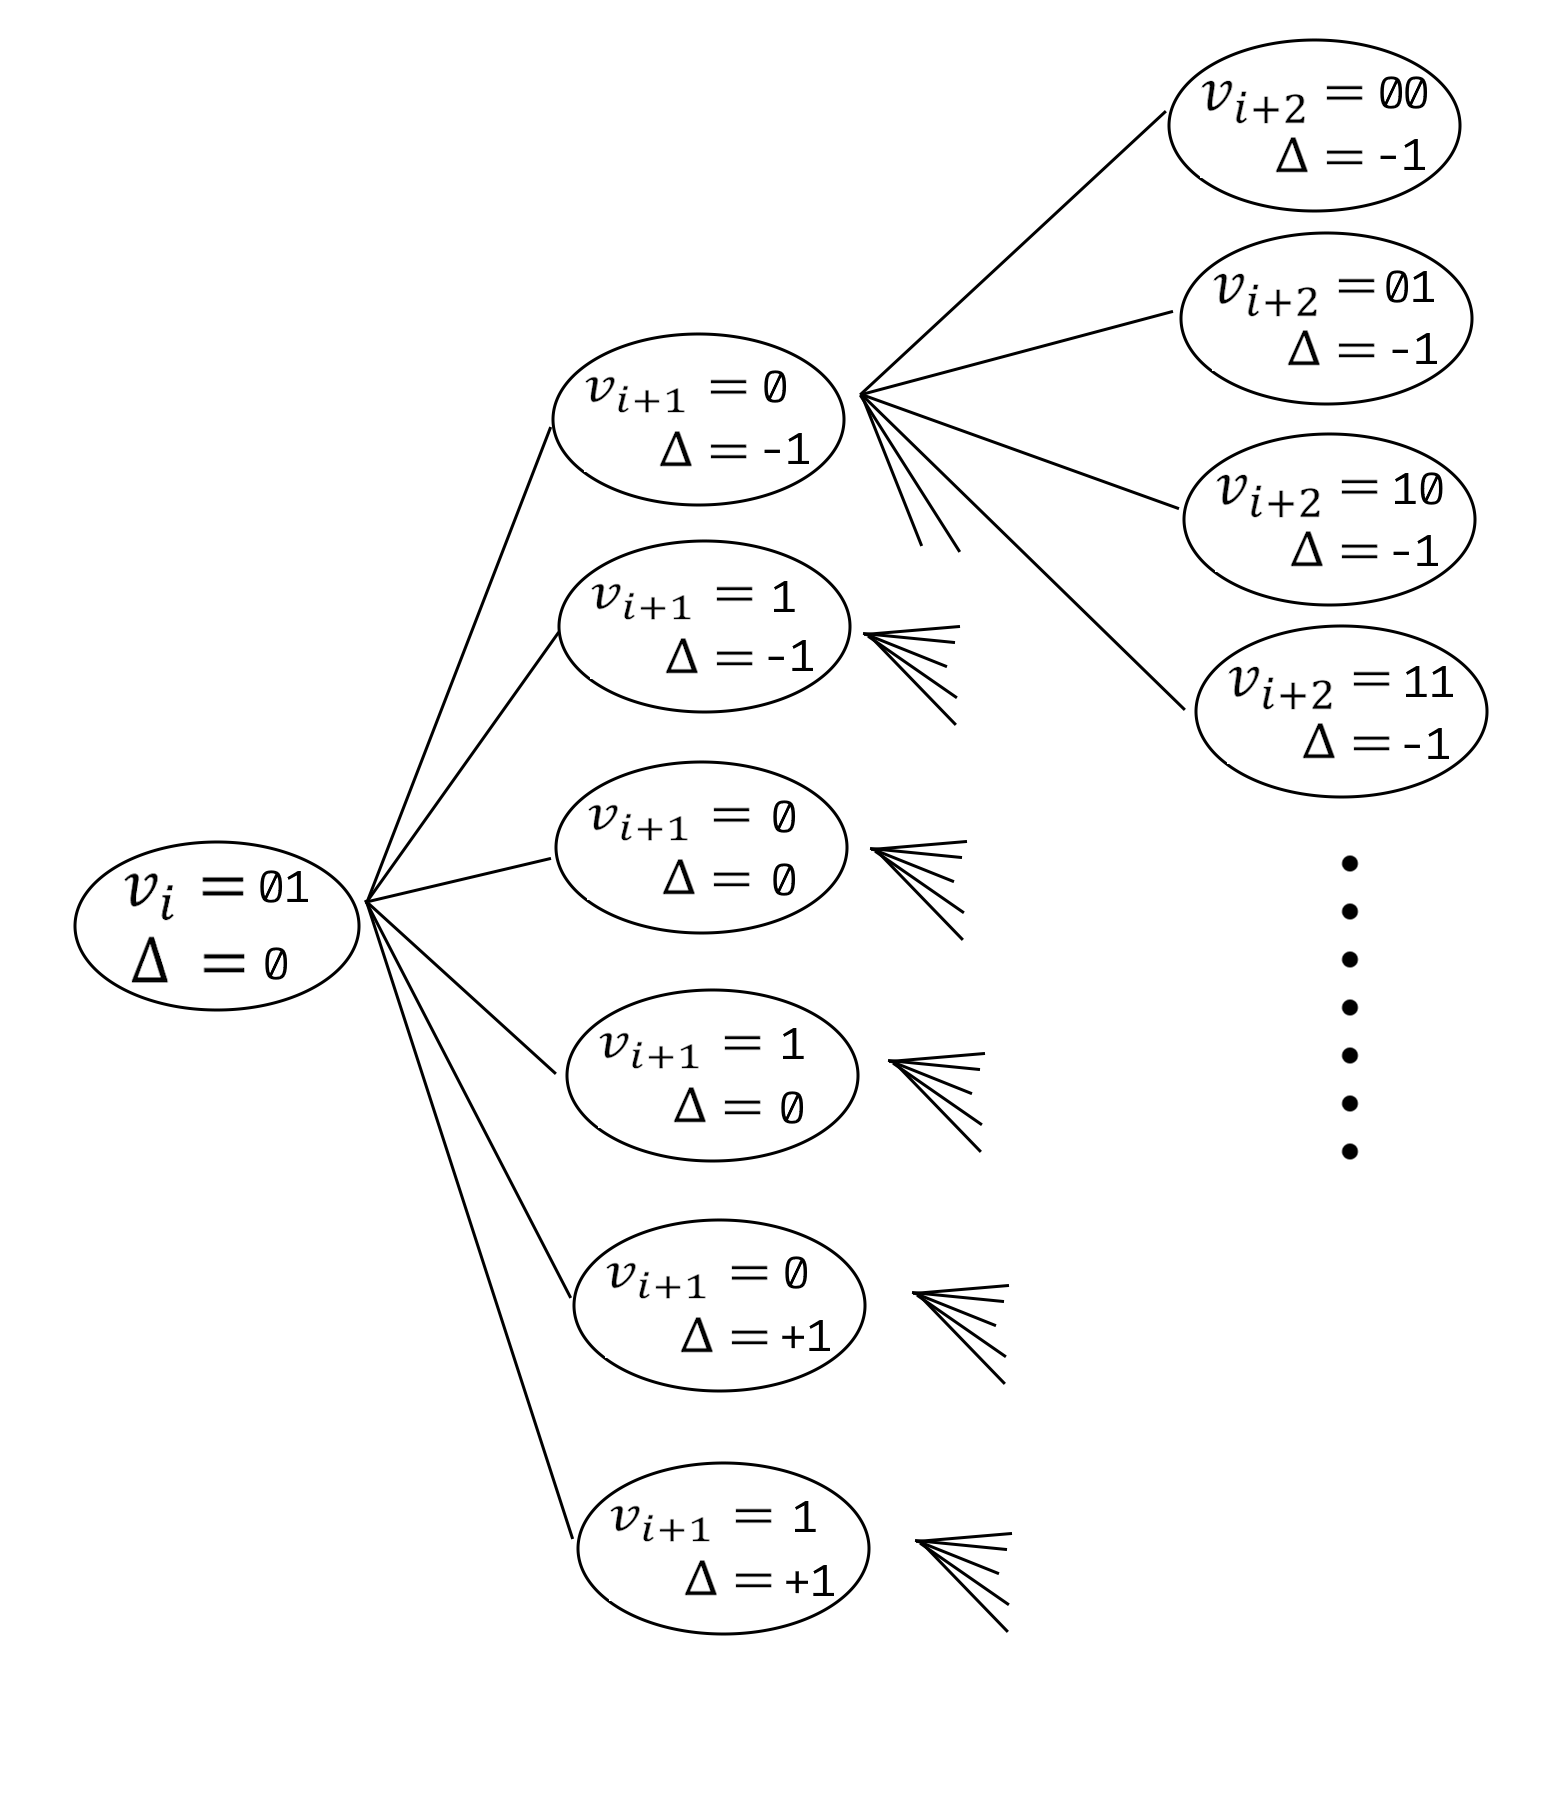
\includegraphics[width=100mm]{heap.png}
    \caption{Heap structure used in HEDGES decoding}\label{fig:heap}
    \end{center}
\end{figure}
In the decoding process, candidate hypotheses are generated for all combinations of $v_i$ and skew $\Delta$,
and are inserted into the heap.
For each hypothesis, the base $C_i$ predicted from $v_i$ using Eq.~\eqref{encode} is compared with the
corresponding input base $C'_i$.
If they match, a reward is added to the score; if they do not match, a penalty is added.
At each step, the hypothesis with the smallest cumulative score is selected as the parent, and its successors
are generated to expand the heap.
Depending on the skew value, the per-step penalty $\Delta P$ is computed using the reward $P_{\mathrm{ok}}$,
substitution penalty $P_{\mathrm{sub}}$, insertion penalty $P_{\mathrm{ins}}$, and deletion penalty
$P_{\mathrm{del}}$ as follows:
\begin{itemize}
  \item $\Delta = 0$: \\ No shift in position; this represents either a correct read or a substitution error.
  \begin{align}
    \Delta P = \begin{cases}
      P_{\mathrm{ok}} & (\text{if bases match}) \\
      P_{\mathrm{sub}} & (\text{if bases do not match})
    \end{cases}
  \end{align}
  \item $\Delta = -1$: \\ A deletion error is hypothesized, and the reference position in the input sequence is
  moved back by one base.
  In this case, there is no base to compare, so only the deletion penalty is applied.
  \begin{align}
    \Delta P = P_{\mathrm{del}}
  \end{align}
  \item $\Delta = 1$: \\ A single-base insertion error is hypothesized, and the reference position in the input
  sequence is advanced by one base.
  \begin{align}
    \Delta P = \begin{cases}
      P_{\mathrm{ins}} + P_{\mathrm{ok}} & (\text{if bases match}) \\
      P_{\mathrm{ins}} + P_{\mathrm{sub}} & (\text{if bases do not match})
    \end{cases}
  \end{align}
\end{itemize}
The score of each hypothesis is obtained by adding $\Delta P$ to the score of its parent hypothesis.
As a result, incorrect hypotheses quickly accumulate large penalties, whereas the correct decoding path
remains with a significantly smaller score than competing paths, enabling efficient identification
of the correct sequence.
Near the end of the message, however, there are not enough subsequent bases for incorrect hypotheses
to accumulate sufficient penalties, and the decoding accuracy tends to degrade.
To mitigate this effect, two bytes of zero-padding, called runout, are appended to the end of the message
during encoding and removed after decoding.

To avoid exponential growth in computational complexity during heap search, an upper bound is imposed on the
heap size.
Once this limit is reached, decoding for that strand is declared to have failed, the search is terminated,
and all remaining bits in the strand are marked as erasures.
These erasures are eventually corrected by the outer RS code.

\subsection{Nanopore Sequencers and Basecallers} \label{nanopore}
Nanopore sequencers determine DNA sequences by exploiting the fact that DNA molecules are charged in
solution and can be driven electrophoretically through nanometer-scale pores in a membrane
\cite{Amarasinghe2020,Dorey2024}.
Figure~\ref{fig:nanopore} illustrates the principle and workflow of nanopore sequencing.
On the sensor substrate called a flow cell, many protein nanopores are embedded, each forming a pore of
approximately 1~nm in diameter through which only a single DNA strand can pass.
The flow cell is filled with an electrolyte solution containing potassium chloride, and DNA molecules in the
solution carry a negative charge.
By applying a voltage across the membrane, an electric field is created that drives the DNA strand toward
the nanopores by electrophoresis.

Once captured by a nanopore, double-stranded DNA is unwound into a single strand by a helicase enzyme and
is translocated through the pore at a controlled speed.
As the DNA strand passes through the pore, it partially blocks the ionic current; the magnitude of the
resulting current depends on the local sequence of bases within the pore at that time.
By measuring and analyzing these current fluctuations over time, the underlying DNA base sequence can be
inferred.
\begin{figure}
    \begin{center}
        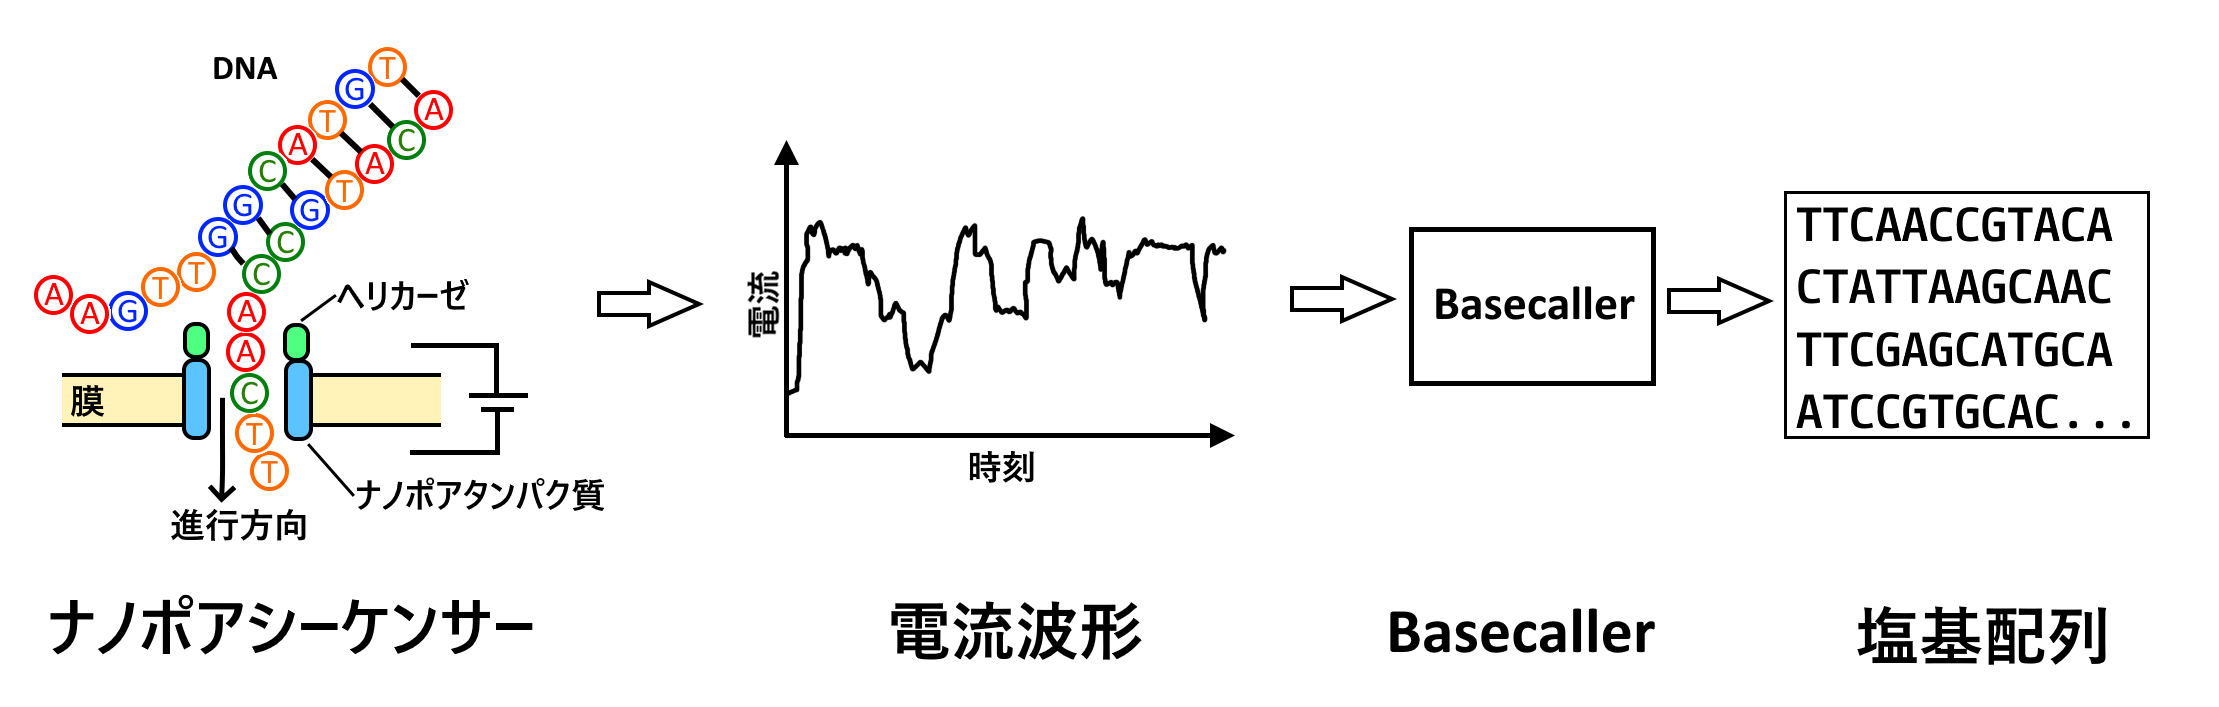
\includegraphics[width=150mm]{nanopore.png}
    \caption{Principle and workflow of nanopore sequencing}\label{fig:nanopore}
    \end{center}
\end{figure}

The process of converting current signals into base sequences is called basecalling and is performed by a
machine-learning model known as a basecaller.
Figure~\ref{fig:bonito} shows the architecture of Bonito, the basecaller used in this study\cite{bonito}.
Bonito first applies a convolutional neural network (CNN) to the input current signal to extract local
features.
It then uses a long short-term memory (LSTM) network to capture long-range temporal dependencies in the
signal.
Finally, a CTC output layer applies a linear transformation to the LSTM outputs and produces, at each time
step, a score vector over the label set \{N,A,C,G,T\}, where N denotes a blank label.
The final base sequence is obtained by applying beam search to this score sequence.
During this process, a post-processing step called Collapse is applied to the label sequences:
\begin{enumerate}
  \item 連続する同一ラベルを1つにまとめる．
  \item 空白ラベル(N)を削除する．
\end{enumerate}
With this procedure, for example, the label sequence ``AANNCCGNGGGTT'' is converted to ``ACGGT''.
\begin{figure}
    \begin{center}
        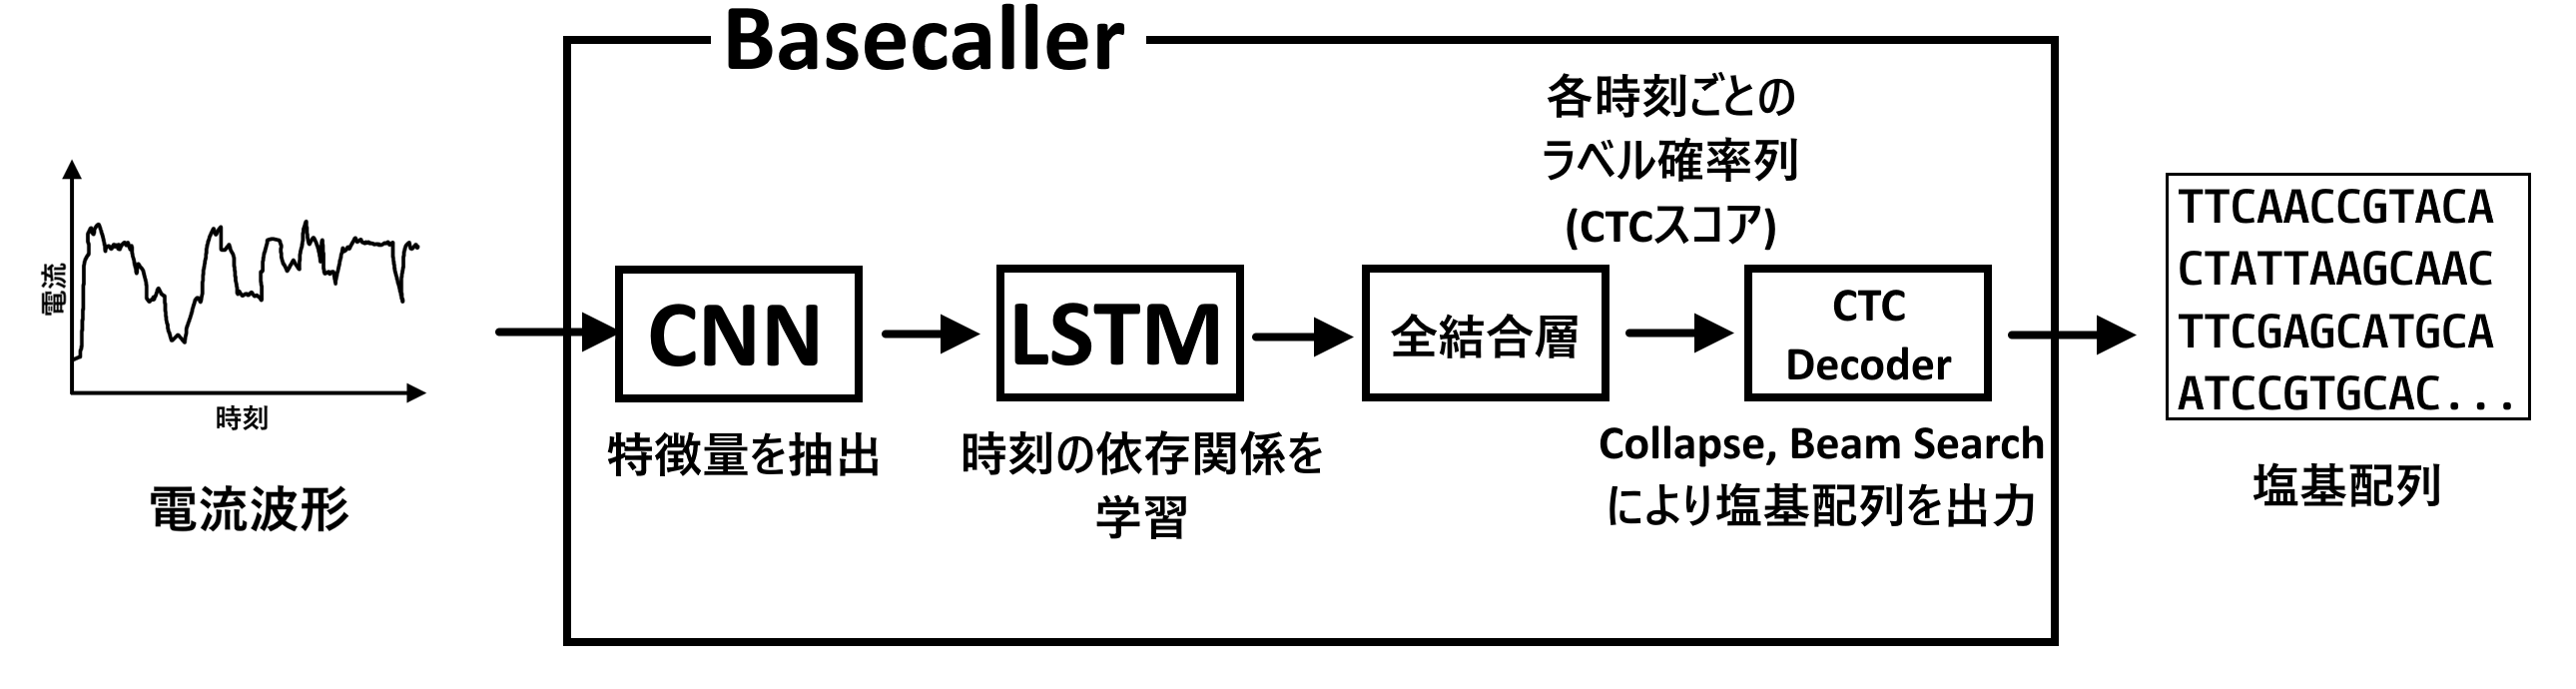
\includegraphics[width=150mm]{architecture.png}
    \caption{Overview of the Bonito architecture}\label{fig:bonito}
    \end{center}
\end{figure}

Using nanopore sequencers for DNA storage readout offers several advantages.
They can directly analyze long DNA strands ranging from hundreds of bp to several megabases in a single run
and provide high-throughput, real-time sequencing.
% 以下のような点が挙げられる\cite{Amarasinghe2020,Dorey2024,SBS}．
% \begin{itemize}
%   \item SBS法では一度に解析できるDNAの塩基長が数十bpから数百bpと短く，塩基長の長いDNAは
%   複数の断片に分割して解析する必要があるのに対し，ナノポアシーケンサーは一度に数百bpから数百万bpの
%   塩基長の長いのDNAを直接的に解析することが出来る．
%   \item SBS法では解析に数日から数週間を要するのに対し，ナノポアシーケンサーは400bp/s
%   での高速な解析が可能である．
%   \item ナノポアシーケンサーはリアルタイムでの解析が可能であり，解析するサンプルを
%   柔軟に制御できるため，必要なデータを効率的に取り出すことが出来る．
%   \item 小型で低コストな装置であるため，設置場所の制約が少なく，運用コストが低い．
% \end{itemize}
On the other hand, accurately controlling the translocation speed of DNA with a helicase is challenging,
and the basecaller does not always infer the correct base sequence from the noisy current signals.
As a result, nanopore sequencers are known to have lower basecalling accuracy than SBS-based short-read
sequencers, particularly with respect to insertion and deletion errors.
Consequently, robust error-correcting codes are especially important when using nanopore sequencers for
DNA storage\cite{Amarasinghe2020,Dorey2024}.

\subsection{Limitations of Existing Methods and Research Objectives} \label{sec:problem}
The work in\cite{HEDGES} has several limitations when applied to nanopore-based DNA storage:
\begin{itemize}
  % \item 既存のHEDGES復号アルゴリズムにおいて，置換・挿入・消失エラーに対する
  % ペナルティ$P_{\mathrm{sub}}$，$P_{\mathrm{ins}}$，$P_{\mathrm{del}}$の値は概念的には各エラーの発生確率の負の対数
  % であるとされているが，先行研究のシミュレーション評価においては，各エラーが等しい確率で
  % 発生する場合を想定して$P_{\mathrm{sub}} = P_{\mathrm{ins}} = P_{\mathrm{del}}=1$と設定した上で，
  % いくつかの符号化率において最適な報酬$P_{\mathrm{ok}}$の値を経験的に決定するにとどめられており，
  \item The rewards and penalties used in the existing HEDGES decoder are not optimized based on the
  statistical readout characteristics of nanopore sequencers.
  \item Because the input to the conventional HEDGES decoder is only a base sequence, it does not exploit
  the full probability distribution over bases output by the basecaller at each time step.
  \item For long DNA strands, the number of hypotheses explored by the existing HEDGES encoder/decoder
  grows rapidly and the heap-size limit is often reached, causing frequent decoding failures and
  degradation in decoding accuracy.
\end{itemize}
In this study, we propose an error-correction method tailored to DNA storage systems that use nanopore
sequencers for readout.
For the rewards and penalties in the HEDGES decoding algorithm, we optimize their values by explicitly
modeling the statistical readout characteristics of nanopore sequencers, such as the error probabilities
and transition probabilities between bases.
We further incorporate the probability distributions over bases output by the basecaller into the reward
and penalty computation, aiming to reduce the search complexity of decoding while improving accuracy.
In addition, we propose an improved encoding scheme that mitigates the degradation in decoding performance
when handling long DNA strands.
The effectiveness of the proposed methods is evaluated through simulations.

\section{Error-Correction Method for Nanopore-Based DNA Storage}\label{proposed_method}
\subsection{Improving Decoding Efficiency} \label{optimization}
In this section, we propose a method for improving the efficiency of the decoding search.
The key idea is to optimize the reward and penalty terms in HEDGES decoding by taking into account both the
statistical readout characteristics of nanopore sequencers and the basewise probability distributions
output by the basecaller at each time step.
We first describe how to model the nanopore readout characteristics and how to handle the CTC output of the
basecaller, and then present a method for incorporating this information into the reward and penalty terms.

\subsubsection{Modeling the Readout Characteristics of Nanopore Sequencers} \label{stat_model}
To model the readout characteristics of nanopore sequencers, we first construct a transition matrix that
represents the statistical error rates.
When both the original DNA sequence and the sequence obtained after readout are known, a sequence-alignment
method can be used to compare the two sequences and identify matches and the locations of various errors
\cite{GOTOH1982705}.
In the aligned pair, positions where the two bases match correspond to correct reads, whereas mismatched
pairs indicate substitution errors.
If a base in one sequence is aligned with a gap in the other, this corresponds to an insertion or deletion error.
Thus, each event in nanopore readout---correct reading or occurrence of substitution, insertion, and deletion errors---
can be expressed as a transition between the five labels $\{N, A, C, G, T\}$, where N denotes a gap (blank) symbol
in addition to the four bases.

Using this view, we represent the statistical readout characteristics of the nanopore sequencer by the
following transition matrix $\bm{T}$:
\begin{align}
  \bm{T} = \begin{bmatrix}
    0 & p_{AN} & p_{CN} & p_{GN} & p_{TN} \\
    p_{NA} & p_{AA} & p_{CA} & p_{GA} & p_{TA} \\
    p_{NC} & p_{AC} & p_{CC} & p_{GC} & p_{TC} \\
    p_{NG} & p_{AG} & p_{CG} & p_{GG} & p_{TG} \\
    p_{NT} & p_{AT} & p_{CT} & p_{GT} & p_{TT} \\
  \end{bmatrix}
\end{align}
Each element in this matrix represents the probability of correct reads and substitution, insertion,
or deletion errors when a sufficiently long DNA sequence with equal base composition is read by the nanopore
sequencer.
For $X,Y \in \{A,C,G,T\}$,
\begin{itemize}
  \item $p_{XX}$: probability that base $X$ is read correctly.
  \item $p_{XY}$: probability that base $X$ is substituted by base $Y$.
  \item $p_{XN}$: probability that base $X$ is deleted.
  \item $p_{NY}$: probability that base $Y$ is inserted.
\end{itemize}
The sum of all elements of $\bm{T}$ is 1.
We define $\bm{P}_{\mathrm{STATS}}$ as the matrix obtained by taking the natural logarithm of each element
of $\bm{T}$ (except the $(1,1)$ element) and multiplying it by $-1$.
The entries of $\bm{P}_{\mathrm{STATS}}$ are used later to compute rewards and penalties.

\subsubsection{Handling CTC Output} \label{ctc_output}
As described in Section~\ref{nanopore}, conventional basecalling applies beam search to the CTC output to produce
the final base sequence.
In the proposed method, however, the basecaller does not commit to a single base sequence; instead, it outputs
the raw CTC score sequence.
Moreover, while the conventional HEDGES decoder in Section~\ref{hedges_decoding} takes only the base sequence as input,
our proposed decoder directly consumes the CTC score sequence (Fig.~\ref{fig:optim}).
This enables the decoding algorithm to exploit the full probability distribution over bases at each time step.
\begin{figure}
    \begin{center}
        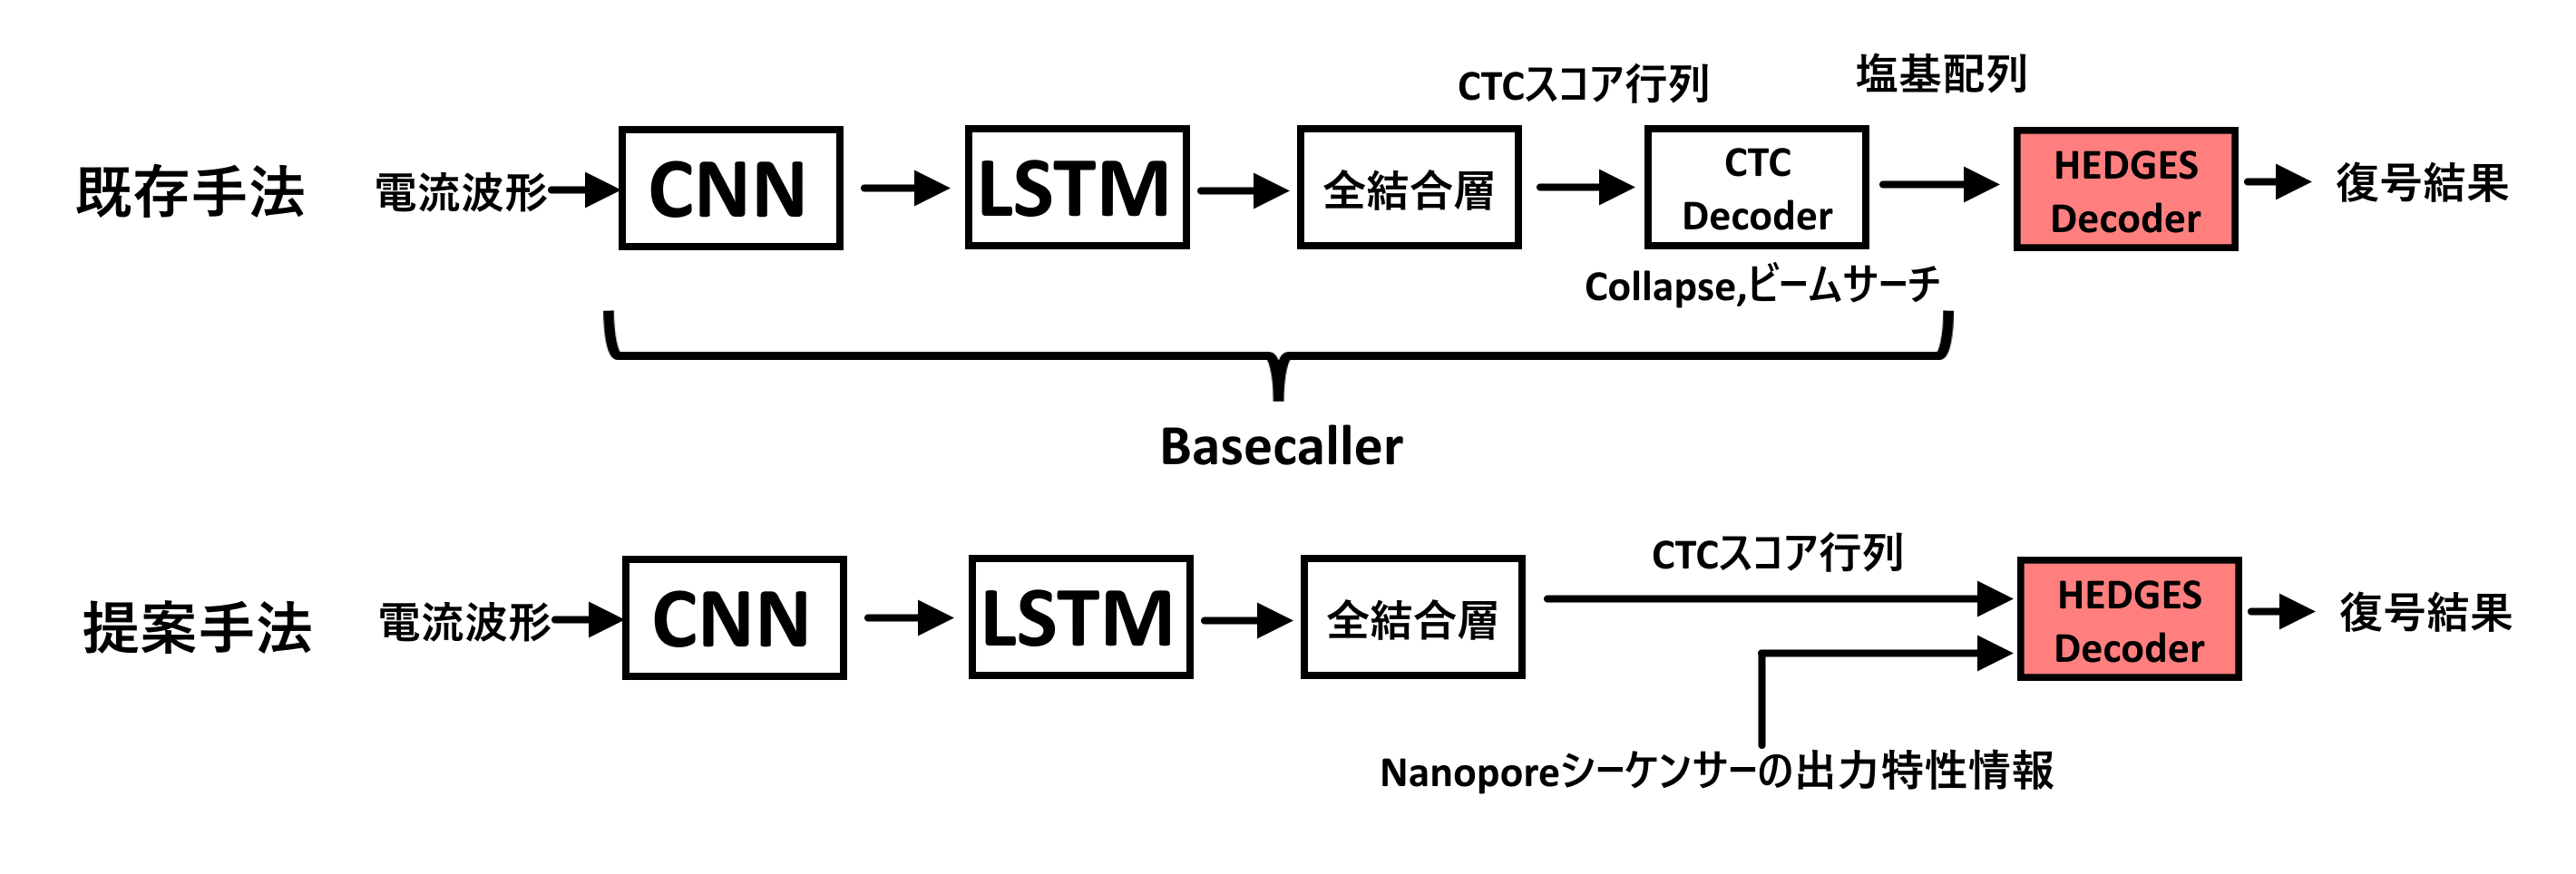
\includegraphics[width=150mm]{optim.png}
        \caption{提案手法の概要}\label{fig:optim}
    \end{center}
\end{figure}

Let the CTC output be given by an $L\times 5$ matrix $\bm{S}$, where $L$ is the length of the current signal
and each row represents the probability distribution over the five labels $\{N,A,C,G,T\}$ at a time step.
We obtain $\bm{S}'$ by applying the following operations to $\bm{S}$, which correspond to the Collapse
step described in Section~\ref{nanopore}:
\begin{enumerate}
  \item For groups of consecutive rows in $\bm{S}$ whose most probable label is identical, we replace them
  with a single row in $\bm{S}'$ whose elements are the average probabilities over the group.
  \item From $\bm{S}'$, we remove rows whose most probable label is the blank symbol N.
\end{enumerate}
% なお，これにより得られた行列$\bm{S}'$の各行で確率が最大となる塩基を選択することで
% 得られる塩基配列は，通常のベースコーラーの最終層でのビームサーチにおいてビーム幅を1と
% した場合のベースコール結果に相当する．
We define $\bm{P}_{\mathrm{CTC}}$ as the matrix obtained by taking the natural logarithm of each element
in $\bm{S}'$ and multiplying it by $-1$.
Each element of $\bm{P}_{\mathrm{CTC}}$ therefore represents a score derived from the probability that a
particular base or blank is output at a given time step.
In the original HEDGES decoder in Section~\ref{hedges_decoding}, the reward or penalty is determined solely
by whether the predicted base (from Eq.~\eqref{encode}) matches the input base.
In the proposed method, we instead obtain the score corresponding to the predicted base from $\bm{P}_{\mathrm{CTC}}$
and use it to adapt the reward and penalty.

\subsubsection{Optimization of Rewards and Penalties} \label{reward_penalty_optimization}
In the original method, the reward $P_{\mathrm{ok}}$ and the penalties for substitution, insertion, and deletion
errors, $P_{\mathrm{sub}}$, $P_{\mathrm{ins}}$, and $P_{\mathrm{del}}$, are fixed constants.
In contrast, we propose new, adaptive reward and penalty terms $P'_{\mathrm{ok}}$, $P'_{\mathrm{sub}}$,
$P'_{\mathrm{ins}}$, and $P'_{\mathrm{del}}$ that incorporate both the nanopore readout statistics in
Section~\ref{stat_model} and the CTC output in Section~\ref{ctc_output}, and define them as
\begin{equation}
  \begin{split}
    P'_{\mathrm{ok}} = P_{\mathrm{ok}} &+ \alpha_{\mathrm{ok}}(\bm{P}_{\mathrm{STATS}}(x_{\mathrm{hypo}}, x_{\mathrm{max}}(i))-\mu_{\mathrm{STATS}\_\mathrm{ok}}) \label{opt1} \\ 
     &+ \beta_{\mathrm{ok}}(\bm{P}_{\mathrm{CTC}}(i, x_{\mathrm{hypo}})-\mu_{\mathrm{CTC}\_\mathrm{ok}}) 
  \end{split}
\end{equation}
\begin{equation}
  \begin{split}
    P'_{\mathrm{sub}} = P_{\mathrm{sub}} &+ \alpha_{\mathrm{sub}}(\bm{P}_{\mathrm{STATS}}(x_{\mathrm{hypo}}, x_{\mathrm{max}}(i))-\mu_{\mathrm{STATS}\_\mathrm{sub}}) \label{opt2} \\
    &+ \beta_{\mathrm{sub}}(\bm{P}_{\mathrm{CTC}}(i, x_{\mathrm{hypo}})-\mu_{\mathrm{CTC}\_\mathrm{sub}})
  \end{split}
\end{equation}
\begin{equation}
  \begin{split}
    P'_{\mathrm{ins}} = P_{\mathrm{ins}} &+ \alpha_{\mathrm{ins}}(\bm{P}_{\mathrm{STATS}}(N, x_{\mathrm{max}}(i-1))-\mu_{\mathrm{STATS}\_\mathrm{ins}}) \label{opt3}\\
    &+ \beta_{\mathrm{ins}}(\bm{P}_{\mathrm{CTC}}(i-1, x_{\mathrm{hypo}})-\mu_{\mathrm{CTC}\_\mathrm{ins}})
  \end{split}
\end{equation}
\begin{equation}
  \begin{split}
    P'_{\mathrm{del}} = P_{\mathrm{del}} &+ \alpha_{\mathrm{del}}(\bm{P}_{\mathrm{STATS}}(x_{\mathrm{hypo}}, N)-\mu_{\mathrm{STATS}\_\mathrm{del}}) \label{opt4}
  \end{split}
\end{equation}
Here, $x_{\mathrm{hypo}}$ denotes the base predicted from the current hypothesis, and $i$ is the row index in
$\bm{P}_{\mathrm{CTC}}$ referenced by the hypothesis.
The symbol $x_{\mathrm{max}}(i)$ denotes the base with the maximum probability in the $i$-th row of $\bm{P}_{\mathrm{CTC}}$.
$\bm{P}_{\mathrm{STATS}}(X,Y)$ $(X,Y\in \{N,A,C,G,T\})$ represents the score corresponding to a transition
from label $X$ to label $Y$ in $\bm{P}_{\mathrm{STATS}}$.
$\bm{P}_{\mathrm{CTC}}(i,X)$ is the score of label $X$ in the $i$-th row of $\bm{P}_{\mathrm{CTC}}$.
$\mu_{\mathrm{STATS}\_\mathrm{ok}}$, $\mu_{\mathrm{STATS}\_\mathrm{sub}}$,
$\mu_{\mathrm{STATS}\_\mathrm{ins}}$, and $\mu_{\mathrm{STATS}\_\mathrm{del}}$ denote the expected scores in
$\bm{P}_{\mathrm{STATS}}$ for correct reads, substitution errors, insertion errors, and deletion errors,
respectively,
% すなわち
% \begin{align}
%   \mu_{\mathrm{STATS}\_\mathrm{ok}} &= \dfrac{\displaystyle \sum_{X \in \{A,C,G,T\}} p_{XX} \bm{P}_{\mathrm{STATS}}(X,X)}{\displaystyle \sum_{X \in \{A,C,G,T\}} p_{XX}} \\
%   \mu_{\mathrm{STATS}\_\mathrm{sub}} &= \dfrac{\displaystyle \sum_{X,Y \in \{A,C,G,T\}, X \neq Y} p_{XY} \bm{P}_{\mathrm{STATS}}(X,Y)}{\displaystyle \sum_{X,Y \in \{A,C,G,T\}, X \neq Y} p_{XY}} \\
%   \mu_{\mathrm{STATS}\_\mathrm{ins}} &= \dfrac{\displaystyle \sum_{Y \in \{A,C,G,T\}} p_{NY} \bm{P}_{\mathrm{STATS}}(N,Y)}{\displaystyle \sum_{Y \in \{A,C,G,T\}} p_{NY}} \\
%   \mu_{\mathrm{STATS}\_\mathrm{del}} &= \dfrac{\displaystyle \sum_{X \in \{A,C,G,T\}} p_{XN} \bm{P}_{\mathrm{STATS}}(X,N)}{\displaystyle \sum_{X \in \{A,C,G,T\}} p_{XN}}
% \end{align}
% である．
while $\mu_{\mathrm{CTC}\_\mathrm{ok}}$, $\mu_{\mathrm{CTC}\_\mathrm{sub}}$, and
$\mu_{\mathrm{CTC}\_\mathrm{ins}}$ denote the expected scores in $\bm{P}_{\mathrm{CTC}}$ for correct reads,
substitution errors, and insertion errors, respectively.
The adaptive reward and penalty terms are computed by adding normalized correction terms, whose expectations
are zero, to the fixed values $P_{\mathrm{ok}}$, $P_{\mathrm{sub}}$, $P_{\mathrm{ins}}$, and $P_{\mathrm{del}}$.
The correction terms are weighted by tuning parameters $\alpha_{\mathrm{ok}}$, $\alpha_{\mathrm{sub}}$,
$\alpha_{\mathrm{ins}}$, $\alpha_{\mathrm{del}}$, $\beta_{\mathrm{ok}}$, $\beta_{\mathrm{sub}}$, and
$\beta_{\mathrm{ins}}$, which are optimized via simulations.
Details on the parameter settings and optimization procedure are provided in the appendix.
% まず，仮説のビット列から出力される塩基を$x_{\mathrm{hypo}}$とする．
% また，仮説が参照する$\bm{P}_{\mathrm{CTC}}$の行番号を$i$とする．
% このとき，$\bm{P}_{\mathrm{CTC}}$の$i$行目において出力確率が最大となる塩基を
% $x_{\mathrm{max}}(i)$とする．

\subsection{Improved Encoding Algorithm for Long Reads} \label{long_read_encoding}
As discussed in Section~\ref{sec:problem}, the decoding accuracy of the conventional HEDGES encoding/decoding
scheme degrades as the DNA strand length increases.
This is because, once the number of hypotheses in the decoder reaches the heap-size limit, decoding is terminated
and all subsequent bits are marked as erasures; longer strands therefore have a higher probability of such failures.
In this section, we propose an improved encoding/decoding algorithm that mitigates this degradation for long reads.

In the original HEDGES encoder, each output base $C_i$ corresponding to $v_i$ is determined by Eq.~\eqref{encode}
using a hash function that depends on the strand ID, bit position, and preceding bits.
As a result, if a burst error occurs at some position on a strand, decoding of all subsequent bases can be affected
through this chaining, making it difficult to recover the correct path.
To address this issue, we divide long DNA sequences into segments of 400~nt as illustrated in Fig.~\ref{fig:segment},
and reinitialize both the bit-position index $I_i$ and the preceding-bit state $B_i$ used by the hash function to zero
at the beginning of each segment.
To locate the segment boundaries during decoding, we insert known separator sequences of about 10 bases between
adjacent segments.
The separators are chosen so that they contain no homopolymers and have a GC content of approximately 50\%.
In this work, we use the sequence ``GTACTGCATG'' as the separator.

During decoding, the separator positions are first detected by the following procedure:
\begin{enumerate}
  \item Set $n=l_{\mathrm{p}} + l_{\mathrm{seg}}$, where $l_{\mathrm{p}}$ is the primer length and
  $l_{\mathrm{seg}}$ is the segment length.
  \item For integers $k$ satisfying $n-30<k<n+30$, compute $S_{\mathrm{match}}(k)$ by
  \begin{align}
    S_{\mathrm{match}}(k) = \sum_{j=0}^{l_{\mathrm{sep}}-1} \bm{P}_{\mathrm{CTC}}(k+j, S_j) \label{eq:separator_detection}
  \end{align}
  where $S_j$ denotes the $j$-th base of the separator sequence and $l_{\mathrm{sep}}$ is the separator length.
  The value $k$ that minimizes $S_{\mathrm{match}}(k)$ is selected as the separator position and denoted by $k'$.
  \item Set $n=k' + l_{\mathrm{sep}}+l_{\mathrm{seg}}$.
  \item Repeat steps~2 and 3 to detect the separator positions of all segments.
\end{enumerate}
Once the separator positions have been identified, we apply the decoder in Section~\ref{hedges_decoding}
to each segment independently.
At the beginning of each segment, both $I_i$ and $B_i$ are reset to zero and the heap is reinitialized.
This approach prevents the heap from exceeding its size limit due to accumulated errors and localizes
decoding failures within individual segments, allowing decoding to resume from the next segment.
\begin{figure}
    \begin{center}
        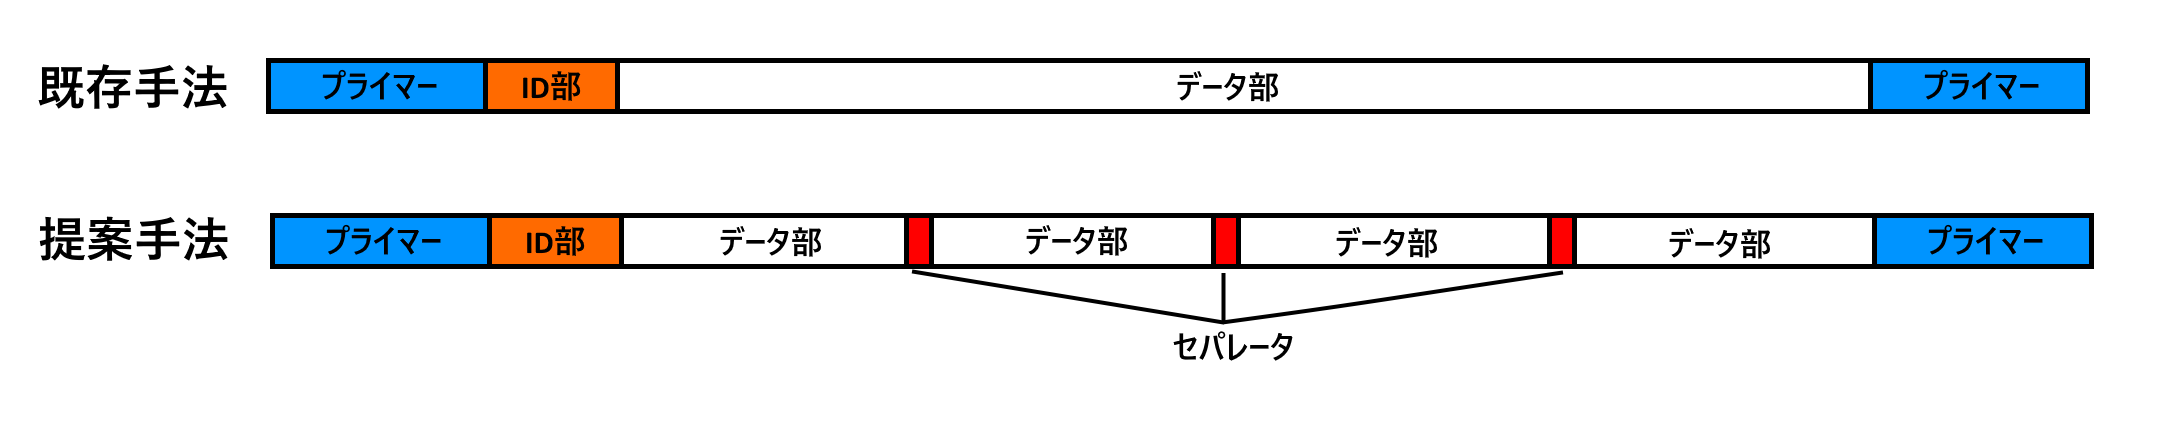
\includegraphics[width=150mm]{segment.png}
        \caption{Proposed segmented encoding scheme}\label{fig:segment}
    \end{center}
\end{figure}

\section{Simulation Results} \label{simulation}
In this chapter, we evaluate the performance of the proposed methods via simulations.
Section~\ref{sim1} assesses the decoding search complexity and accuracy when applying the reward/penalty
optimization of Section~\ref{optimization}, and compares the results with those of the baseline method.
Section~\ref{sim2} evaluates the decoding accuracy of the improved long-read encoding/decoding algorithm
of Section~\ref{long_read_encoding} and compares it with the conventional approach.

\subsection{Decoding Search Efficiency} \label{sim1}
\subsubsection{Experimental Setup}
Figure~\ref{fig:sim1} summarizes the simulation flow used to evaluate the performance of the proposed
reward and penalty optimization in Section~\ref{optimization}.
\begin{figure}
    \begin{center}
        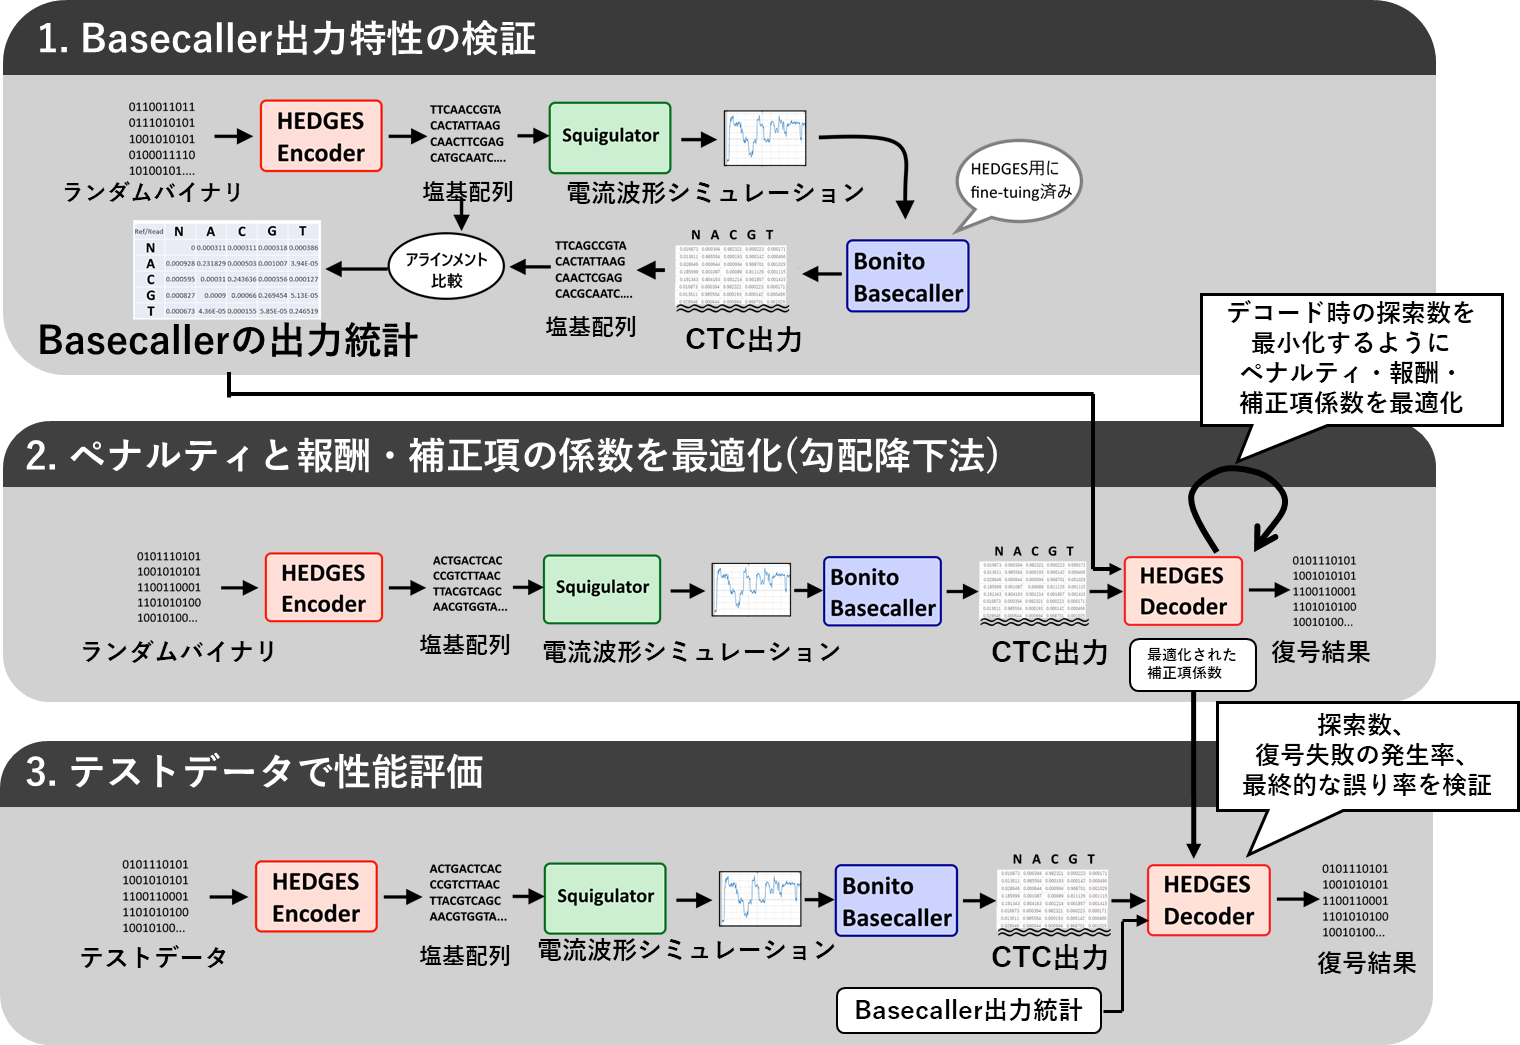
\includegraphics[width=150mm]{simu1.png}
        \caption{Overview of the simulation flow}\label{fig:sim1}
    \end{center}
\end{figure}
As a preliminary step, we estimated the nanopore readout statistics via simulation and obtained
the matrix $\bm{P}_{\mathrm{STATS}}$.
Next, using encoding/decoding simulations with random binary data, we optimized the parameters of the
correction terms in Eqs.~\eqref{opt1}--\eqref{opt4} by gradient descent, using the heap search count during
decoding as the objective function.
The parameter optimization was performed independently for each code rate and for three configurations:
using only the nanopore-based correction terms, using only the CTC-based terms, and using both.
Details of this preliminary experiment, including conditions and implementation, are provided in the appendix.

Using the optimized parameters obtained above, we evaluated the decoding performance of the proposed method.
The test binary data were first encoded with HEDGES, and the resulting DNA sequences were passed to
Squigulator\cite{squigulator} to simulate nanopore current signals.
The simulated signals were then basecalled by Bonito, which was configured to output both the final base sequence
and the CTC score matrix before decoding.
Using these basecalling results, we ran both the baseline decoder and the proposed decoders and measured
the heap search count, the number of erased bits due to decoding failures, and the final bit error rate
after RS decoding.
In the baseline decoder, only the base sequence output by the basecaller was used.
In the proposed decoders, the CTC score matrix was used as input and three configurations were evaluated:
using only the nanopore-statistics-based correction terms, using only the CTC-based terms, and using both.
These end-to-end simulations from binary encoding to final decoding were performed for multiple code rates.

\subsubsection{Experimental Conditions}
As test data, we used the full text (UTF-8) of ``Kokoro'' by Natsume S\={o}seki obtained from Aozora Bunko,
after removing ruby annotations (text enclosed in 《…》) using regular expressions\cite{kokoro}.
The resulting file size was 481,158~bytes.
This binary data was encoded by HEDGES with code rates $0.75, 0.60, 0.50, 0.33$ and DNA strand length 400~nt.
For current-signal simulation with Squigulator, we used parameter settings corresponding to the MinION R9.4.1
flow cell\cite{squigulator}.
The Bonito model was obtained by fine-tuning a publicly available pre-trained model
on HEDGES-encoded DNA readout data\cite{bonito}.
For both the baseline and proposed decoders, the heap size limit was set to 1,000,000.

\subsubsection{Results and Discussion}
Tables~\ref{tab:results_heap}, \ref{tab:results_deletion}, and \ref{tab:results_final_ber} summarize,
respectively, the average heap search count per DNA strand, the bit-erasure rate due to decoding failures,
and the final bit error rate after RS decoding.
In these tables,
the row ``STATS only'' indicates that only the nanopore-statistics-based correction terms were applied,
``CTC only'' indicates that only the CTC-based correction terms were applied, and ``STATS+CTC'' indicates
that both types of corrections were used.
\begin{table}
  \centering
  \caption{Average heap search count per DNA strand}
  \label{tab:results_heap}
  \begin{tabular}{c|c|cccc}
    \hline
    \multicolumn{2}{c|}{Code rate} & 0.75 & 0.6 & 0.5 & 0.33 \\
    \hline
    \multicolumn{2}{c|}{Baseline} & 135550 & 45219 & 21291 & 12290 \\
    \hline
    \multirow{3}{*}{Proposed} & STATS only & 77281 & 23707 & 10893 & 4785 \\
    \cline{2-6}
     & CTC only & 53098 & 17966 & 9353 & 4354 \\
    \cline{2-6}
     & STATS+CTC & 48507 & 14972 & 7625 & 3894 \\
    \hline
  \end{tabular}
\end{table}
\begin{table}
  \centering
  \caption{Bit-erasure rate due to decoding failures}
  \label{tab:results_deletion}
  \begin{tabular}{c|c|cccc}
    \hline
    \multicolumn{2}{c|}{Code rate} & 0.75 & 0.6 & 0.5 & 0.33 \\
    \hline
    \multicolumn{2}{c|}{Baseline} & 0.03083 & 0.00949 & 0.00341 & 0.00328 \\
    \hline
    \multirow{3}{*}{Proposed} & STATS only & 0.00741 & 0.00376 & 0.00121 & 0.00076 \\
    \cline{2-6}
     & CTC only & 0.00789 & 0.00265 & 0.00111 & 0.00055 \\
    \cline{2-6}
     & STATS+CTC & 0.00693 & 0.00229 & 0.00069 & 0.00056 \\
    \hline
  \end{tabular}
\end{table}
\begin{table}
  \centering
  \caption{Bit error rate after RS decoding}
  \label{tab:results_final_ber}
  \begin{tabular}{c|c|cccc}
    \hline
    \multicolumn{2}{c|}{Code rate} & 0.75 & 0.6 & 0.5 & 0.33 \\
    \hline
    \multicolumn{2}{c|}{Baseline} & 0.022981 & $<10^{-6}$ & $<10^{-6}$ & $<10^{-6}$ \\
    \hline
    \multirow{3}{*}{Proposed} & STATS only & 0.059977 & $<10^{-6}$ & $<10^{-6}$ & $<10^{-6}$ \\
    \cline{2-6}
     & CTC only & 0.008228 & $<10^{-6}$ & $<10^{-6}$ & $<10^{-6}$ \\
    \cline{2-6}
     & STATS+CTC & 0.005173 & $<10^{-6}$ & $<10^{-6}$ & $<10^{-6}$ \\
    \hline
  \end{tabular}
\end{table}
The proposed methods significantly reduced both the heap search count and the decoding failure rate for all
code rates compared with the baseline.
When only the nanopore-statistics-based correction terms were applied, the heap search count was reduced by
43--61\%, and the bit-erasure rate was reduced by 60--77\%.
When only the CTC-based correction terms were used, the heap search count was reduced by 56--65\% and the
bit-erasure rate by 68--83\%.
When both types of correction terms were applied, the heap search count was further reduced by 64--68\%, and
the bit-erasure rate by 76--83\%, yielding the best overall performance.
Furthermore, for code rate 0.75, applying both corrections reduced the final bit error rate after RS decoding
by 77\% compared with the baseline.
These results demonstrate that the proposed optimization not only improves decoding efficiency but also
reduces the occurrence of decoding failures, thereby contributing to improved end-to-end reliability.

\subsection{Improved Long-Read Encoding and Decoding} \label{sim2}
\subsubsection{Experimental Setup}
To evaluate the performance of the improved long-read encoding/decoding algorithm proposed in
Section~\ref{long_read_encoding}, we compared the conventional, non-segmented method with the proposed
segmented method by simulation, measuring both decoding search complexity and accuracy.

First, we encoded test binary data using the original HEDGES encoder.
The resulting DNA sequences were then passed through the same current-signal simulation and basecalling
pipeline as in Section~\ref{sim1}.
Using these basecalling results, we applied the proposed decoder of Section~\ref{optimization}, with
parameters fixed to the values obtained in Section~\ref{sim1}, while varying the strand length between
500~nt and 15,000~nt.
For each strand length, we measured the bit error rate of HEDGES decoding.
For the conventional method, we evaluated two cases: (1) a fixed heap-size limit independent of strand length,
and (2) a heap-size limit that scales proportionally with the strand length.

Next, using the same binary data, we encoded the sequences with the proposed segmented scheme and again
performed current-signal simulation and basecalling.
During decoding, separator positions were first detected using $\bm{P}_{\mathrm{CTC}}$ obtained by the
procedure in Section~\ref{ctc_output}, following the method described in Section~\ref{long_read_encoding}.
We then applied the proposed decoder of Section~\ref{optimization} to each segment.
Keeping the segment length fixed, we varied the number of segments so that the overall strand length ranged
from about 500~nt to 15,000~nt and measured the bit error rate of HEDGES decoding.

\subsubsection{Experimental Conditions}
The test binary data were the same as those used in Section~\ref{sim1}.
The Squigulator parameter settings for current-signal simulation and the basecaller model were also identical
to those in Section~\ref{sim1}.
Both the conventional and proposed schemes used a code rate of 0.60.
In the proposed segmented scheme, the segment length was fixed to 400~nt.
For the conventional method, we evaluated (1) a fixed heap-size limit of 1,000,000 regardless of strand length,
and (2) a heap-size limit that was proportional to strand length, normalized so that the limit was 1,000,000
for 400~nt.
For the proposed method, the heap-size limit was set to 1,000,000 for each segment.

\subsubsection{Results and Discussion}
Figure~\ref{fig:long_read_results1} shows the relationship between DNA strand length and bit error rate,
and Fig.~\ref{fig:long_read_results2} shows the relationship between strand length and the average heap
search count per strand.
Here, ``Conventional (1)'' corresponds to the fixed heap-size limit, and ``Conventional (2)'' to the
length-proportional heap-size limit.
Consistent with the results reported in\cite{HEDGES}, for Conventional (1) the bit error rate increased
almost linearly with strand length.
For Conventional (2), increasing the heap-size limit in proportion to strand length kept the bit error rate
approximately constant, but resulted in the largest heap search counts among the three methods.
In contrast, for the proposed segmented method, the bit error rate remained almost unchanged even as the strand
length increased.
Because the heap-size limit of the proposed method is applied per segment, the total heap search count per strand
was about 24\% larger than that of Conventional (1), but about 21\% smaller than that of Conventional (2).

These observations suggest that the degradation of decoding accuracy in the conventional method is primarily
caused by the increased decoding failure rate associated with the growth in heap search complexity.
By reinitializing both the hash-function state and the heap at every segment, the proposed method can limit
the heap size while localizing decoding failures to individual segments and continuing decoding from later
segments, thereby suppressing the overall accuracy degradation for long reads.
\begin{figure}
  \centering
  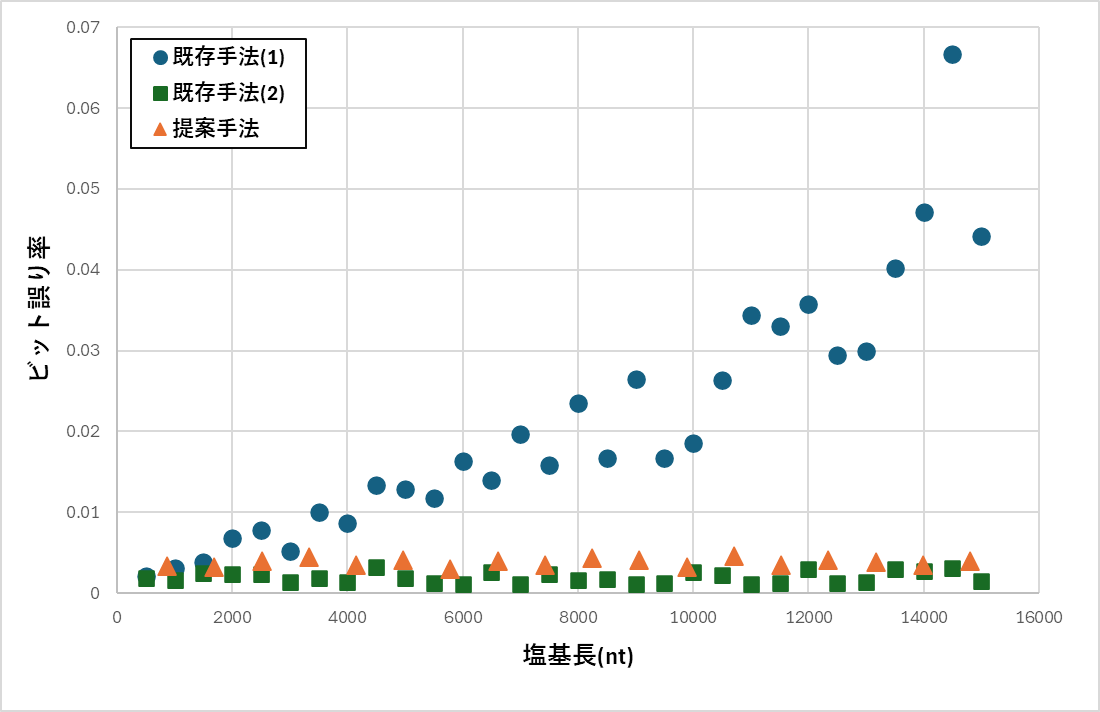
\includegraphics[width=120mm]{longread1.png}
  \caption{Relationship between strand length and bit error rate}
  \label{fig:long_read_results1}
\end{figure}
\begin{figure}
  \centering
  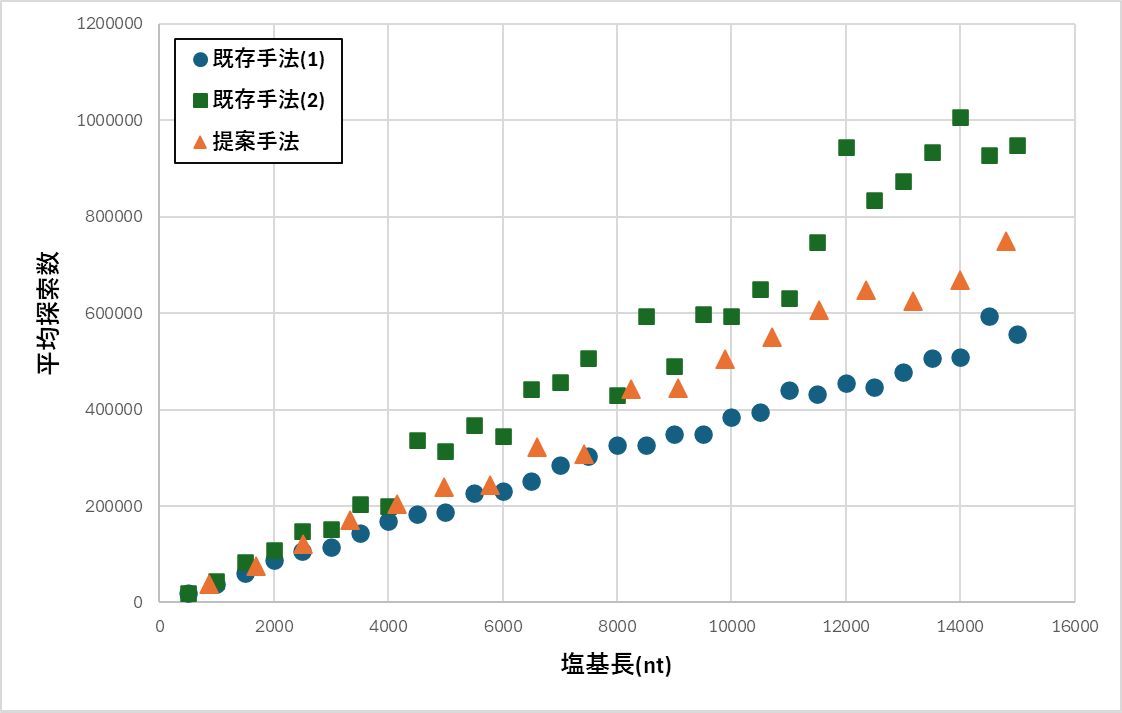
\includegraphics[width=120mm]{longread2.png}
  \caption{Relationship between strand length and average heap search count per strand}
  \label{fig:long_read_results2}
\end{figure}
\section{Conclusion}
In this work, we proposed an error-correction method for DNA storage systems that use nanopore sequencers
for readout and evaluated its performance by simulation.
HEDGES, the baseline scheme, is an error-correcting code that satisfies DNA sequence constraints and is robust
to insertion, deletion, and substitution errors.
However, its decoding algorithm is not optimized for nanopore-based readout, and its decoding accuracy
degrades for long DNA strands.

To address these issues, we first proposed a decoding strategy that incorporates both the statistical readout
characteristics of nanopore sequencers and the CTC output of the basecaller into the HEDGES decoding process.
Experimental results showed that, compared with the baseline method, the proposed optimization reduced the
heap search count by 64--68\% and the bit-erasure rate due to decoding failures by 76--83\%.
We then proposed an improved encoding/decoding algorithm for long reads based on segmentation and demonstrated
that it effectively suppresses the degradation of decoding accuracy for long DNA strands.

Several directions remain for future work.
First, the nanopore readout model can be refined.
In this study we used a relatively simple model that considers only label transition probabilities.
Incorporating more detailed characteristics, such as context dependence on neighboring bases and bursty error
patterns, may allow further optimization of decoding.
Second, it is important to support state-of-the-art basecaller architectures.
While we used Bonito, which adopts a CNN--LSTM--CTC topology, recent basecallers employ more advanced models
such as CTC/CRF hybrids; adapting the proposed framework to these models is expected to further improve
decoding accuracy.
Third, experimental validation with real DNA is needed.
Because our evaluation is based solely on simulations, it is necessary to perform nanopore sequencing
experiments on synthesized DNA encoded by HEDGES to confirm the practical effectiveness of the proposed method.


%======================================================================
%		謝辞
%======================================================================
\begin{acknowledgements}
The author would like to express sincere gratitude to Prof. Takafumi Sato for his
continuous guidance and insightful advice throughout this research.
The author is also deeply grateful to Assoc. Prof. Hiromitsu Awano, Prof. Masayoshi Hashimoto,
Assoc. Prof. Rei Ueno, Assist. Prof. Ryo Shirai, Prof. Keiichi Niitsu, and Assist. Prof. Kunyang Liu
for their valuable comments and suggestions in seminars and meetings.
Special thanks are due to Mr. Takefumi Koike for many helpful discussions and advice on daily research.
The author also thanks Ms. Shuko Nishiyama and Ms. Kaori Uenishi, the administrative staff of the Sato Laboratory,
for their kind support in many aspects of laboratory life.
Finally, the author would like to thank all members of the Sato, Hashimoto, and Niitsu laboratories
for their constant encouragement and support.
\end{acknowledgements}



%======================================================================
%		参考文献
%======================================================================
\bibliographystyle{kueethesis}
\bibliography{reference}



%======================================================================
%		付録
%======================================================================
\appendix
\section{Preliminary Experiments on Improving Decoding Search Efficiency}
\subsection{Experimental Method}
First, to obtain the matrix $\bm{P}_{\mathrm{STATS}}$ representing the readout characteristics of
the nanopore sequencer, we encoded randomly generated binary data into multiple DNA strands using
HEDGES and simulated the ionic-current waveforms of nanopore sequencing with Squigulator.
Next, we applied Bonito to the simulated waveforms to obtain the CTC output and computed
$\bm{P}_{\mathrm{CTC}}$ by the method described in Section~\ref{ctc_output}.
Here, let $C_i^{(j)}$ denote the $i$th base of the $j$th DNA strand in the HEDGES-encoded result,
and let $\{C_i^{(j)}\}$ denote the corresponding base sequence.
Let $\bm{P}_{\mathrm{CTC}}^{(j)}$ denote the CTC output matrix obtained by basecalling
$\{C_i^{(j)}\}$, and let $\{C'^{{(j)}}_i\}$ denote the base sequence obtained by selecting,
for each row of $\bm{P}_{\mathrm{CTC}}^{(j)}$, the base with the maximum output probability.
We performed global alignment between $\{C'^{{(j)}}_i\}$ and $\{C_i^{(j)}\}$ and counted,
for each base, the occurrences of correct reads and substitution, insertion, and deletion errors
\cite{GOTOH1982705}.
Repeating this procedure for all $j$ and aggregating the results, we obtained the occurrence
probabilities of each event and thus the matrix $\bm{P}_{\mathrm{STATS}}$.

Because $\mu_{\mathrm{STATS}\_\mathrm{ok}}$, $\mu_{\mathrm{STATS}\_\mathrm{sub}}$,
$\mu_{\mathrm{STATS}\_\mathrm{ins}}$, and $\mu_{\mathrm{STATS}\_\mathrm{del}}$ denote the expected
scores of $\bm{P}_{\mathrm{STATS}}$ for correct reads, substitution errors, insertion errors, and
deletion errors, respectively, they can be computed as
\begin{align}
  \mu_{\mathrm{STATS}\_\mathrm{ok}} &= \dfrac{\displaystyle \sum_{X \in \{A,C,G,T\}} p_{XX} \bm{P}_{\mathrm{STATS}}(X,X)}{\displaystyle \sum_{X \in \{A,C,G,T\}} p_{XX}} \\
  \mu_{\mathrm{STATS}\_\mathrm{sub}} &= \dfrac{\displaystyle \sum_{X,Y \in \{A,C,G,T\}, X \neq Y} p_{XY} \bm{P}_{\mathrm{STATS}}(X,Y)}{\displaystyle \sum_{X,Y \in \{A,C,G,T\}, X \neq Y} p_{XY}} \\
  \mu_{\mathrm{STATS}\_\mathrm{ins}} &= \dfrac{\displaystyle \sum_{Y \in \{A,C,G,T\}} p_{NY} \bm{P}_{\mathrm{STATS}}(N,Y)}{\displaystyle \sum_{Y \in \{A,C,G,T\}} p_{NY}} \\
  \mu_{\mathrm{STATS}\_\mathrm{del}} &= \dfrac{\displaystyle \sum_{X \in \{A,C,G,T\}} p_{XN} \bm{P}_{\mathrm{STATS}}(X,N)}{\displaystyle \sum_{X \in \{A,C,G,T\}} p_{XN}}
\end{align}
Similarly, because $\mu_{\mathrm{CTC}\_\mathrm{ok}}$, $\mu_{\mathrm{CTC}\_\mathrm{sub}}$, and
$\mu_{\mathrm{CTC}\_\mathrm{ins}}$ denote the expected scores of $\bm{P}_{\mathrm{CTC}}$ for correct
reads, substitution errors, and insertion errors, respectively, they are given by
\begin{align}
  \mu_{\mathrm{CTC}\_\mathrm{ok}} &= \dfrac{1}{M}\sum_j \sum_i \bm{P}_{\mathrm{CTC}}^{(j)}(i, C'^{(j)}_i) \\
  \mu_{\mathrm{CTC}\_\mathrm{sub}} &= \dfrac{1}{3M}\sum_j \sum_i \sum_{X \in \{A,C,G,T\}, X \neq C'^{(j)}_i} \bm{P}_{\mathrm{CTC}}^{(j)}(i, X) \\
  \mu_{\mathrm{CTC}\_\mathrm{ins}} &= \dfrac{1}{M}\sum_j \sum_i \bm{P}_{\mathrm{CTC}}^{(j)}(i, N)
\end{align}
where $M$ denotes the total number of bases over all basecalled DNA strands.

Next, we determined the optimal values of the fixed rewards and penalties
$P_{\mathrm{ok}}, P_{\mathrm{sub}}, P_{\mathrm{ins}}, P_{\mathrm{del}}$ in
Eqs.~\eqref{opt1}--\eqref{opt4} and the weighting parameters of the correction terms
$\alpha_{\mathrm{ok}}, \alpha_{\mathrm{sub}}, \alpha_{\mathrm{ins}}, \alpha_{\mathrm{del}},
\beta_{\mathrm{ok}}, \beta_{\mathrm{sub}}, \beta_{\mathrm{ins}}$.
Here, for $P_{\mathrm{ok}}$ we used, for each code rate, the values adopted in
\cite{HEDGES} and optimized all other parameters.
The optimization of these parameters was performed by gradient descent using numerical
differentiation, with the number of heap searches during decoding as the objective function.
Specifically, we first encoded randomly generated binary data using HEDGES, simulated nanopore
readout, applied the basecaller to the resulting current waveforms, and obtained the CTC output.
The parameter optimization by gradient descent was then carried out for the decoding of this
CTC output according to the following procedure:
\begin{enumerate}
    \item Initialize each parameter to be optimized with an appropriate initial value.
    \item Perform decoding using the proposed method and measure the number of heap searches
      required until decoding completes.
    \item For each parameter, add a small perturbation $\Delta$ and again measure the number
      of heap searches during decoding.
    \item Compute the gradient of the objective function with respect to each parameter using
      these values.
    \item Update each parameter using the learning rate $\eta$ as
  \begin{align}
    \bm{\theta} \leftarrow \bm{\theta} - \eta \dfrac{\partial J}{\partial \bm{\theta}}
  \end{align}
  where $\bm{\theta}$ denotes the vector of parameters to be optimized and $J$ is the
  objective function.
  \item Repeat steps 2--5 a fixed number of times.
\end{enumerate}
For parameter optimization, to evaluate the effect of using both the nanopore-statistics-based
and CTC-based correction terms as well as each type alone, we not only optimized the 10 parameters
$P_{\mathrm{sub}}$, $P_{\mathrm{ins}}$, $P_{\mathrm{del}}$, $\alpha_{\mathrm{ok}}$,
$\alpha_{\mathrm{sub}}$, $\alpha_{\mathrm{ins}}$, $\alpha_{\mathrm{del}}$,
$\beta_{\mathrm{ok}}$, $\beta_{\mathrm{sub}}$, and $\beta_{\mathrm{ins}}$, but also conducted
experiments where only six parameters were optimized with
$\alpha_{\mathrm{ok}}=\alpha_{\mathrm{sub}}=\alpha_{\mathrm{ins}}=\alpha_{\mathrm{del}}=0$,
and where only seven parameters were optimized with
$\beta_{\mathrm{ok}}=\beta_{\mathrm{sub}}=\beta_{\mathrm{ins}}=0$.
These optimizations were performed independently for each code rate
$0.75, 0.60, 0.50,$ and $0.33$.

\subsection{Experimental Conditions}
In the simulation to obtain the matrix $\bm{P}_{\mathrm{STATS}}$, we encoded 400~KB of randomly
generated binary data with HEDGES at a code rate of 0.50.
The base length of each DNA strand was set to 400~nt, and a total of 12,240 DNA strands were
generated.
The parameter settings of Squigulator for current-signal simulation and the basecaller model
were identical to those used in the experiment of Section~\ref{sim1}.

For fine-tuning the basecaller, we used 200~KB of randomly generated binary data encoded by
HEDGES at a code rate of 0.50 and base length 400~nt, resulting in 6,120 DNA strands, together
with their simulated current waveforms obtained by Squigulator, as training data.
Starting from the weights of the pre-trained model dna\_r9.4.1@v2, we trained with a batch size
of 64 for 75 steps per epoch and performed 50 epochs of fine-tuning.

For alignment between $\{C^{(n)}_i\}$ and $\{C'^{(n)}_i\}$, we used the global alignment
implementation of the Gotoh algorithm in Biopython
\cite{biopython,GOTOH1982705}.

For parameter optimization, we used the CTC outputs obtained by applying current-signal
simulation and basecalling to HEDGES-encoded DNA strands generated from 400~KB of randomly
generated binary data at code rates $0.75, 0.60, 0.50,$ and $0.33$ with base length 400~nt.
For $P_{\mathrm{ok}}$, we used the fixed values listed in
Table~\ref{tab:fixed_reward} for each code rate.
The initial values of the parameters were set to
$P_{\mathrm{sub}}=P_{\mathrm{ins}}=P_{\mathrm{del}}=1.0$,
$\alpha_{\mathrm{ok}}=\alpha_{\mathrm{sub}}=\alpha_{\mathrm{ins}}=\alpha_{\mathrm{del}}=0.0$, and
$\beta_{\mathrm{ok}}=\beta_{\mathrm{sub}}=\beta_{\mathrm{ins}}=0.0$.
The learning rates listed in Table~\ref{tab:learning_rate} were used for each code rate, and the
parameters were updated 300 times.
\begin{table}
  \centering
  \begin{minipage}{0.48\linewidth}
    \centering
    \caption{Fixed reward values $P_{\mathrm{ok}}$ for each code rate}
    \label{tab:fixed_reward}
    \begin{tabular}{c|c}
      \hline
      Code rate & $P_{\mathrm{ok}}$ \\
      \hline
      0.75 & -0.035 \\
      0.60 & -0.082 \\
      0.50 & -0.127 \\
      0.33 & -0.229 \\
      \hline
    \end{tabular}
  \end{minipage}
  \hfill
  \begin{minipage}{0.48\linewidth}
    \centering
    \caption{Learning rate $\eta$ for each code rate}
    \label{tab:learning_rate}
    \begin{tabular}{c|c}
      \hline
      Code rate & $\eta$ \\
      \hline
      0.75 & $1.3 \times 10^{-7}$ \\
      0.60 &  $4.1 \times 10^{-7}$\\
      0.50 &  $1.0 \times 10^{-6}$ \\
      0.33 &  $3.8 \times 10^{-6}$ \\
      \hline
    \end{tabular}
  \end{minipage}
\end{table}
Note that the random binary data used for the simulation to obtain $\bm{P}_{\mathrm{STATS}}$, for
fine-tuning the basecaller, and for parameter optimization were all generated independently.

\subsection{Results}
The transition probabilities between labels $\{N,A,C,G,T\}$ obtained from evaluating the
readout characteristics of the nanopore sequencer are shown in
Table~\ref{tab:transition_matrix}.
\begin{table}
  \centering
  \caption{Transition probabilities between labels}
  \label{tab:transition_matrix}
  \begin{tabular}{c|ccccc}
    \hline
    Input$\backslash$Output & N & A & C & G & T \\
    \hline
    N & $0.000$ & $3.11 \times 10^{-4}$ & $3.11 \times 10^{-4}$ & $3.18 \times 10^{-4}$ & $3.86 \times 10^{-4}$  \\
    A & $9.28 \times 10^{-4}$ & $0.232$ & $5.03 \times 10^{-4}$ & $1.01 \times 10^{-3}$ & $3.94 \times 10^{-5}$ \\
    C & $5.95 \times 10^{-4}$ & $3.10 \times 10^{-4}$ & $0.244$ & $3.56 \times 10^{-4}$ & $1.27 \times 10^{-4}$ \\
    G & $8.27 \times 10^{-4}$ & $9.00 \times 10^{-4}$ & $6.60 \times 10^{-4}$ & $0.269$ & $5.13 \times 10^{-5}$ \\
    T & $6.73 \times 10^{-4}$ & $4.36 \times 10^{-5}$ & $1.55 \times 10^{-4}$ & $5.85 \times 10^{-5}$ & $0.247$ \\
    \hline
  \end{tabular}
\end{table}
From these results, correct reads accounted for 99.1\% of all events, whereas substitution,
insertion, and deletion errors occurred at rates of 0.421\%, 0.133\%, and 0.302\%, respectively.
Substitution errors tended to occur more frequently between A and G and between C and T.
In particular, substitutions between A and G were found to occur with a probability about 23 times
higher than that between A and T, which had the lowest probability.
The bias in substitution error rates across bases is considered to stem from the similarity in
chemical structure between purine bases (A,G) and pyrimidine bases (C,T)
\cite{10.1371/journal.pone.0257521}.
Insertion errors, represented by transitions from N to A, C, G, or T, occurred with nearly the
same probability for each base.
Deletion errors, represented by transitions from A, C, G, or T to N, occurred at relatively
higher probabilities for A and G than for C and T.
The resulting matrix $\bm{P}_{\mathrm{STATS}}$ is given in Eq.~\eqref{eq:appendix_P_STATS}.
The expected values of each correction term are summarized in
Table~\ref{tab:appendix_mu_values}, and the optimized penalties and weighting parameters of the
correction terms for each code rate are listed in
Tables~\ref{tab:appendix_params_p} and \ref{tab:appendix_params_alpha_beta}.
\begin{align}
  \bm{P}_{\mathrm{STATS}} =
  \begin{bmatrix}
    -1.20 & -0.650 & -0.650 & -0.643 & -0.613 \\
    -0.580 & 0.130 & -0.670 & -0.590 & -1.25 \\
    -0.620 & -0.650 & 0.110 & -0.640 & -1.09 \\
    -0.550 & -0.520 & -0.590 & 0.160 & -1.53 \\
    -0.590 & -1.53 & -1.09 & -1.25 & 0.120 \\
  \end{bmatrix} \label{eq:appendix_P_STATS}
\end{align}

\begin{table}
  \centering
  \caption{Obtained expected values}
  \label{tab:appendix_mu_values}
  \begin{tabular}{c|c}
    \hline
    Parameter & Value \\
    \hline
    $\mu_{\mathrm{STATS}\_\mathrm{ok}}$ & 1.38 \\
    $\mu_{\mathrm{STATS}\_\mathrm{sub}}$ & 7.52 \\
    $\mu_{\mathrm{STATS}\_\mathrm{ins}}$ & 8.01 \\
    $\mu_{\mathrm{STATS}\_\mathrm{del}}$ & 7.17 \\
    $\mu_{\mathrm{CTC}\_\mathrm{ok}}$ & 0.111 \\
    $\mu_{\mathrm{CTC}\_\mathrm{sub}}$ & 6.85 \\
    $\mu_{\mathrm{CTC}\_\mathrm{ins}}$ & 2.78 \\
    \hline
  \end{tabular}
\end{table}

\begin{table}
  \centering
  \caption{Optimized penalty values for each code rate}
  \label{tab:appendix_params_p}
  \footnotesize
  \begin{tabular}{c|c|ccc}
    \hline
    Code rate & Method & $P_{\mathrm{sub}}$ & $P_{\mathrm{ins}}$ & $P_{\mathrm{del}}$ \\
    \hline
    \multirow{3}{*}{0.75} & STATS only$^{*}$ & 0.630 & 0.650 & 0.687 \\
    & CTC only$^{**}$ & 0.837 & 0.912 & 0.765 \\
    & STATS+CTC$^{***}$ & 0.875 & 0.911 & 0.778 \\
    \hline
    \multirow{3}{*}{0.60} & STATS only$^{*}$ & 0.883 & 0.965 & 0.995 \\
    & CTC only$^{**}$ & 0.856 & 1.06 & 0.890 \\
    & STATS+CTC$^{***}$ & 1.08 & 1.17 & 1.02 \\
    \hline
    \multirow{3}{*}{0.50} & STATS only$^{*}$ & 0.988 & 1.17 & 1.25 \\
    & CTC only$^{**}$ & 0.953 & 1.11 & 1.04 \\
    & STATS+CTC$^{***}$ & 1.15 & 1.23 & 1.19 \\
    \hline
    \multirow{3}{*}{0.33} & STATS only$^{*}$ & 1.07 & 1.25 & 1.39 \\
    & CTC only$^{**}$ & 1.06 & 1.22 & 1.21 \\
    & STATS+CTC$^{***}$ & 1.29 & 1.35 & 1.34 \\
    \hline
  \end{tabular}
  
  \small
  \vspace{0.3cm}
  
  \noindent
  \begin{tabular}{@{}l@{}}
    $^{*}$STATS only: uses only correction terms based on the nanopore readout statistics \\
    $^{**}$CTC only: uses only correction terms based on the CTC output \\
    $^{***}$STATS+CTC: uses correction terms based on both the nanopore readout statistics and the CTC output
  \end{tabular}
\end{table}

\begin{table}
  \centering
  \caption{Optimized weighting parameters of the correction terms for each code rate}
  \label{tab:appendix_params_alpha_beta}
  \footnotesize
  \begin{tabular}{c|c|cccc|ccc}
    \hline
    Code rate & Method & $\alpha_{\mathrm{ok}}$ & $\alpha_{\mathrm{sub}}$ & $\alpha_{\mathrm{del}}$ & $\alpha_{\mathrm{ins}}$ & $\beta_{\mathrm{ok}}$ & $\beta_{\mathrm{sub}}$ & $\beta_{\mathrm{ins}}$ \\
    \hline
    \multirow{3}{*}{0.75} & STATS only& 0.0605 & 0.116 & 0.0929 & 0.0952 & 0.00 & 0.00 & 0.00 \\
    & CTC only& 0.00 & 0.00 & 0.00 & 0.00 & -0.192 & 0.211 & 0.347 \\
    & STATS+CTC& 0.00668 & 0.130 & -0.0105 & 0.544 & -0.150 & 0.181 & 0.301 \\
    \hline
    \multirow{3}{*}{0.60} & STATS only & 0.00513 & 0.256 & 0.200 & 0.0969 & 0.00 & 0.00 & 0.00 \\
    & CTC only & 0.00 & 0.00 & 0.00 & 0.00 & -0.223 & 0.190 & 0.419 \\
    & STATS+CTC & 0.110 & 0.243 & 0.236 & 0.219 & -0.115 & 0.184 & 0.330 \\
    \hline
    \multirow{3}{*}{0.50} & STATS only & 0.0548 & 0.294 & 0.0800 & 0.0871 & 0.00 & 0.00 & 0.00 \\
    & CTC only & 0.00 & 0.00 & 0.00 & 0.00 & -0.108 & 0.193 & 0.411 \\
    & STATS+CTC & 0.131 & 0.292 & 0.234 & 0.176 & -0.136 & 0.188 & 0.467 \\
    \hline
    \multirow{3}{*}{0.33} & STATS only & -0.00773 & 0.282 & 0.167 & 0.246 & 0.00 & 0.00 & 0.00 \\
    & CTC only & 0.00 & 0.00 & 0.00 & 0.00 & 0.0272 & 0.145 & 0.422 \\
    & STATS+CTC & 0.0260 & 0.328 & 0.177 & 0.230 & 0.0417 & 0.134 & 0.460 \\
    \hline
  \end{tabular}
\end{table}


\end{document}
% Local Variables:
% fill-column: 70
% End:
